\section{Phase 3: Entwicklung des API Usability Analyzers}
\label{sec:apiua}

Der \textit{\acrfull{apiua}} (siehe Abbildungen \ref{fig:apiua-splash} und \ref{fig:apiua-opencoding-devel}) ist das Werkzeug, mit dessen Hilfe ich die von mir erhobenen und im vorangegangenen Abschnitt beschriebenen Daten analysiert und die im nächsten Kapitel vorgestellten Forschungsergebnisse erarbeitet habe.

Dabei war das Werkzeug zunächst als reine Visualisierungslösung für die spezielle Form der \textit{Programmierfortschritte}-Datenquelle gedacht. Erst durch die Notwendigkeit, die \gls{gtm} direkt dieser Software anwenden zu können, kam sukzessive die Unterstützung der verschiedenen Aktivitäten dieser Forschungsmethode, wie die verschiedenen Kodierungsarten, hinzu. Eine Einführung in die \gls{gtm} findet sich im \sref{sec:gtm}. Die Entwicklung von \gls{apiua} im zeitlichen Verlauf ist im \sref{sec:verlauf} dargestellt.

Der \acrlong{apiua} besteht aus den folgenden drei Komponenten:
\begin{description}
  \item[API Usability Analyzer] wird vom Forscher für die eigentliche Forschungsarbeit verwendet.\footnote{\url{https://github.com/bkahlert/api-usability-analyzer}}
  \item[API Usability Analyzer Client] läuft auf den Arbeitsplätzen der Probanden und ist für die klientseitige Datenerhebung zuständig. Diese Komponente wird genauer online\footnote{\url{https://github.com/bkahlert/api-usability-analyzer-client-python}} und im \sref{sec:apiua-client} beschrieben.
  \item[API Usability Analyzer Server] sammelt die durch Clients erhobenen objektiven Rohdaten, die dann, mit Hilfe des Datenanalysewerkzeugs, verarbeitet werden können. Diese Komponente wird genauer online\footnote{\url{https://github.com/bkahlert/api-usability-analyzer-server-java-ee}} und im \sref{sec:apiua-server} beschrieben.
\end{description}

Dieser Abschnitt beschränkt sich auf das von mir entwickelte Datenanalysewerkzeug selbst. \aref{app:apiua} ergänzt diese Beschreibung, durch eine nähere Erläuterung einzelner Komponenten.

\begin{figure}[ht!]
  \centering
    
\includegraphics[width=0.4\linewidth]{Figures/apiua/splash.png}
  \caption[APIUA: Startbildschirm]{Der Startbildschirm von \gls{apiua}}
  \label{fig:apiua-splash}
\end{figure}

\newgeometry{inner=2cm,outer=1.5cm,top=1.5cm,bottom=1.5cm}
\thispagestyle{empty}
\begin{landscape}
\begin{figure}
  \centering
    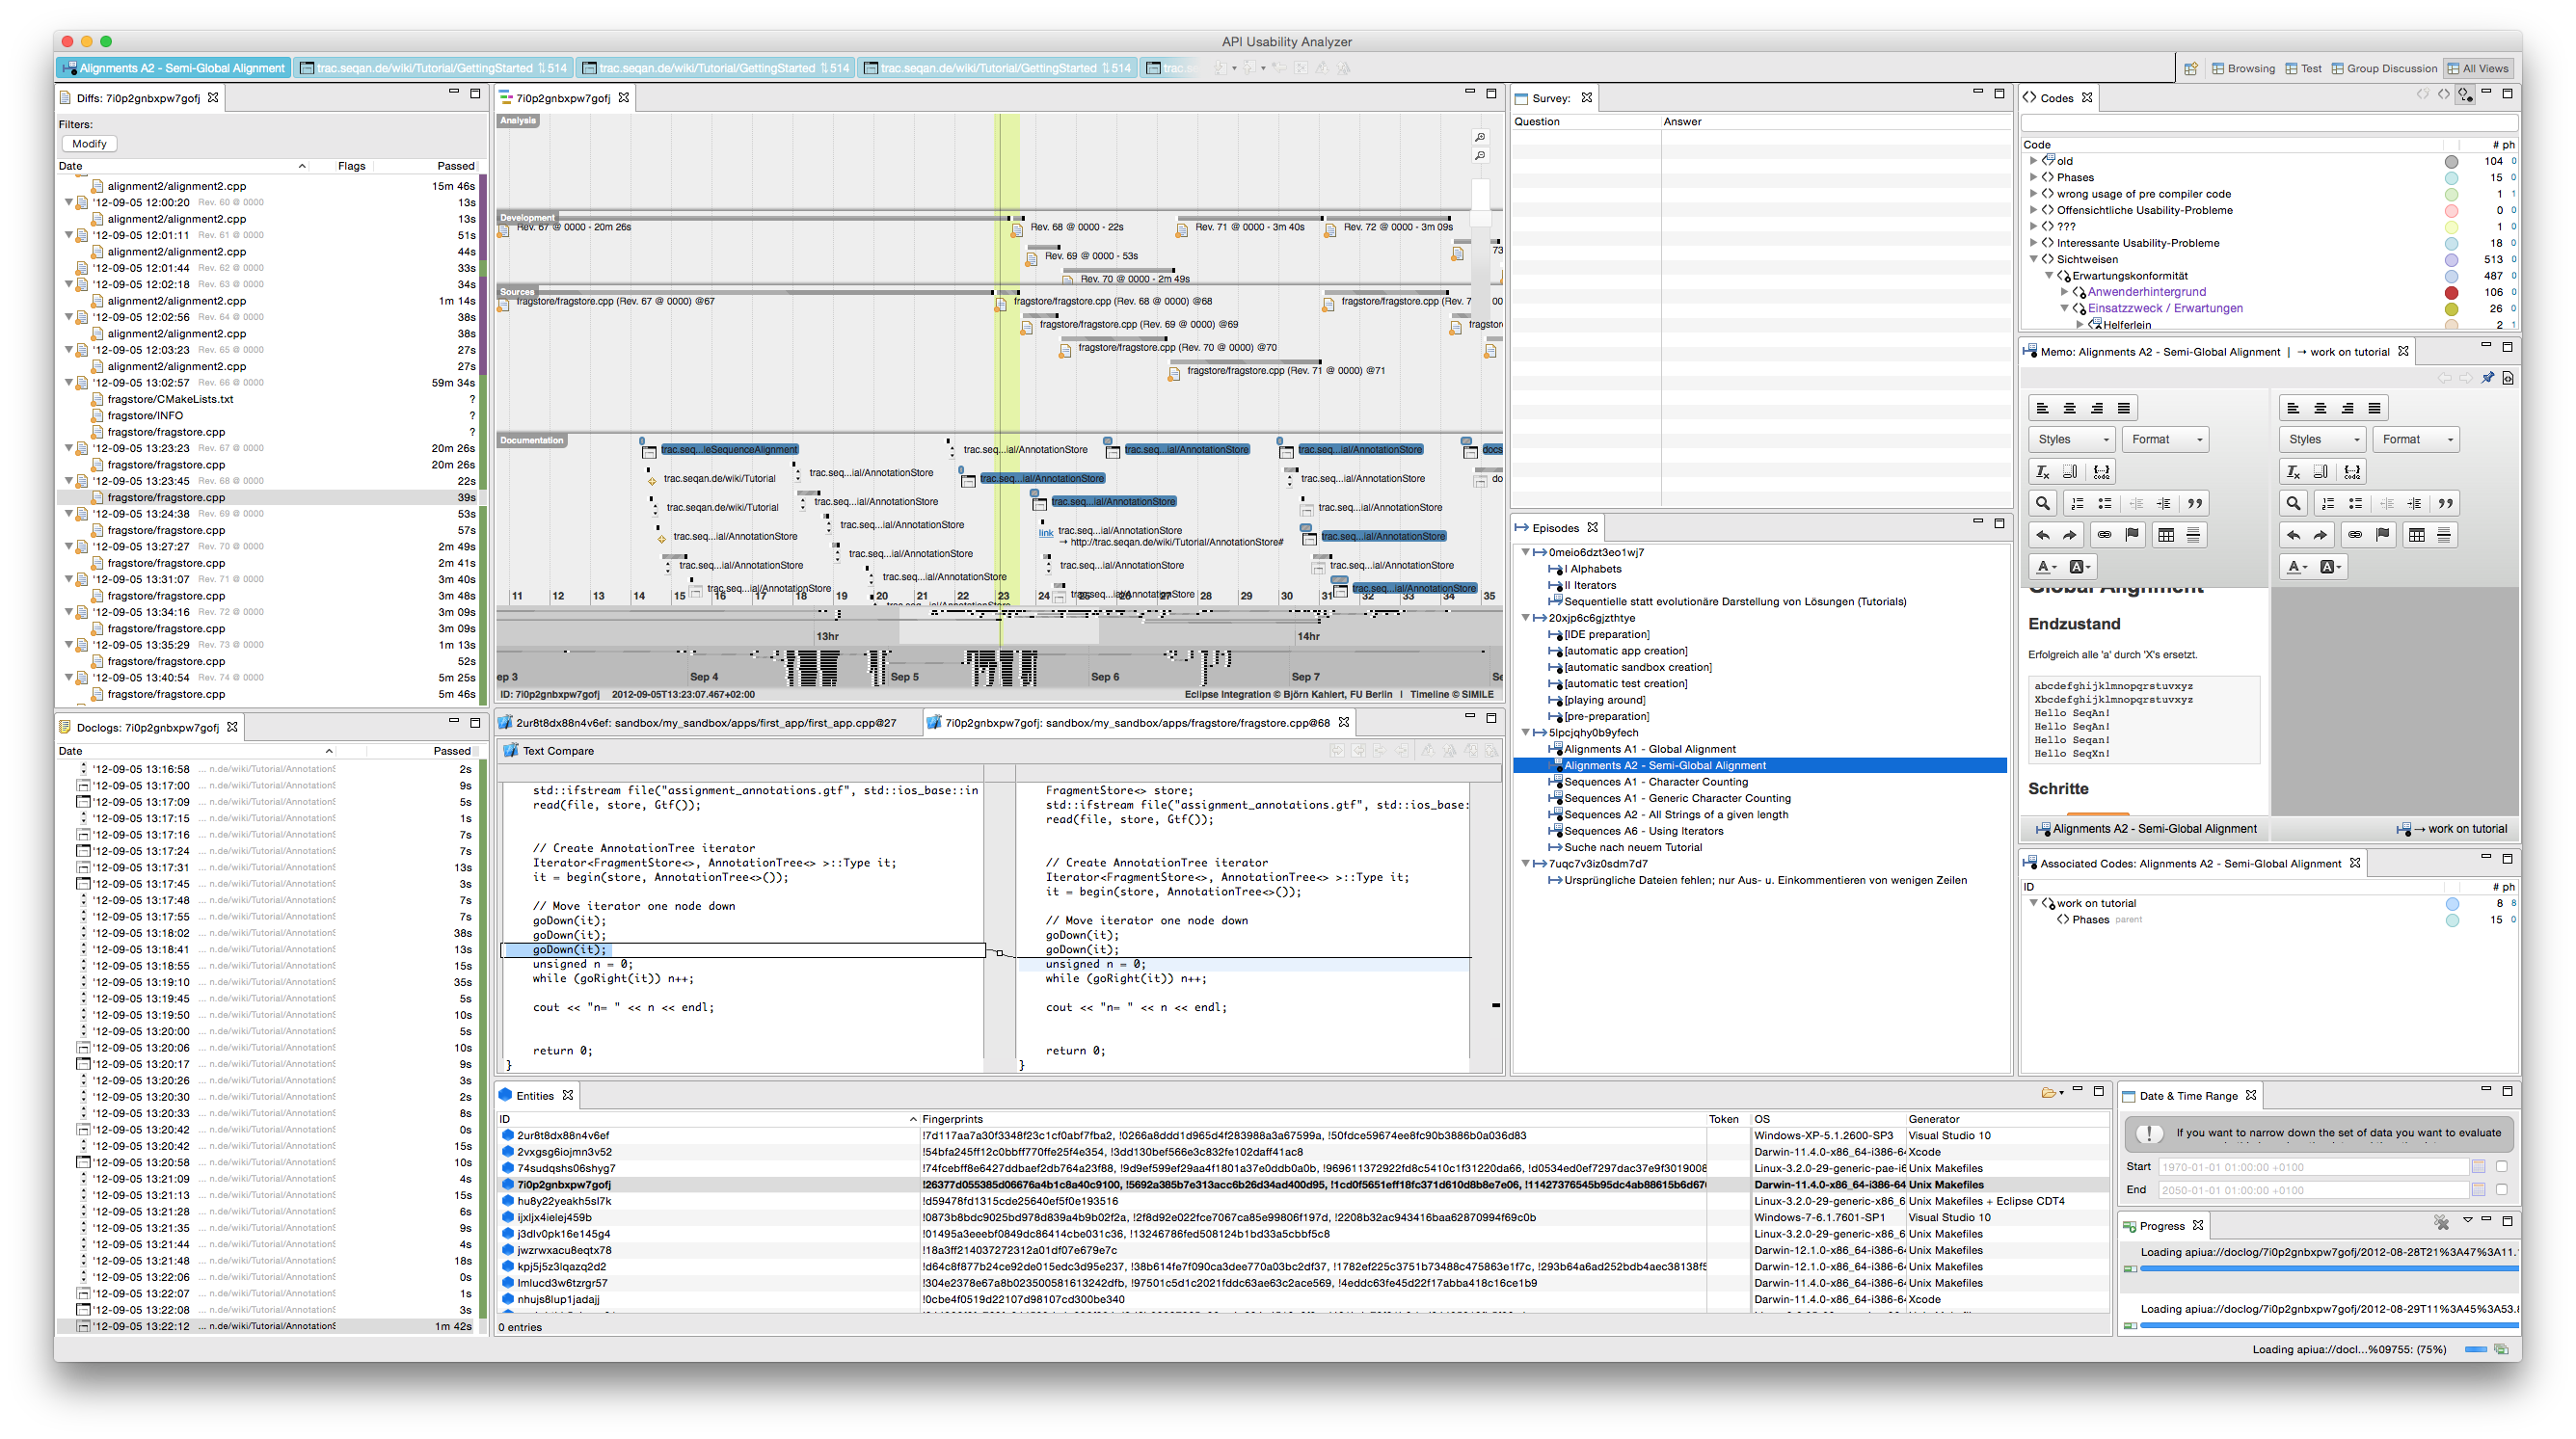
\includegraphics[width=1.0\linewidth]{Figures/apiua/opencoding-devel.png}
  \caption[APIUA: Offenes Kodieren]{Dieser Screenshot von \gls{apiua} zeigt eine typische Sitzung mit Fokus auf offenes Kodieren. In diesem Fall werden Programmierfortschritte des Probanden mit der ID \texttt{7i0p2gnbxpw7gofj} analysiert.}
  \label{fig:apiua-opencoding-devel}
\end{figure}
\end{landscape}
\restoregeometry






\subsection{Motivation}

Je umfassender ein zu analysierendes Datenmaterial ist, desto mehr zwängt sich ein computergestütztes Verfahren auf. Auf dem Markt gibt es verschiedene Anwendungen, die sich grundsätzlich für die Verwendung der \gls{gtm} eignen. Zu den führenden \textit{CAQDAS}\footnote{Computer-unterstützte qualitative Datenanalysesoftware\\(\textit{\textbf{c}omputer \textbf{a}ssisted/\textbf{a}ided \textbf{q}ualitative \textbf{d}ata \textbf{a}nalysis \textbf{s}oftware})}-Vertretern gehören \textit{MAXQDA}\footnote{\url{http://www.MAXQDA.de}} und \textit{ATLAS.ti}\footnote{\url{http://atlasti.com/de/}} \citep{ann2007using}. Beide Programme dienen dem Zweck der qualitativen Datenanalyse und eignen sich für die \gls{gtm} \citep{Wolf:2014vv,Dresing:2006te,ann2007using}.

Bedauerlicherweise haben alle großen CAQDAS-Vertreter nicht zu vernachlässigende Schwächen in Bezug auf ihren Einsatz als \gls{gtm}-Software \citep{ann2007using}. Axiales Kodieren wird von \textit{MAXQDA} überhaupt nicht \citep{Wolf:2014vv} und von anderen Werkzeugen nur im Umfang einer Zeichenfläche unterstützt \citep{ann2007using}. Im letzteren Fall verlieren, auf eine Zeichenfläche positionierte Kodes sogar die Information, woher sie kommen und werden --- im Falle von Kode-Änderungen --- nicht mehr aktualisiert . Einzig \textit{ATLAS.ti} speichert die Referenz auf eine verwendete Relation in ihrem Netzwerk-Editor \citep{ann2007using}. Bezüglich \textit{ATLAS.ti} schildern meine Arbeitsgruppenkollegen \cite{Schenk:3LdEjzOu} und \cite{Zieris:yCXyxVc9} die folgenden Probleme bei ihrer Forschungsarbeit:

\begin{description}
  \item[Funktionale Probleme] \hfill
  \begin{itemize}
    \item Offenes Kodieren wird erschwert, weil Kodes nur sehr eingeschränkt\footnote{Mit Hilfe von Superkodes, Familien und Superfamilien gibt es eine Möglichkeit der Gruppierung \citep{MuhlmeyerMentzel:2011vs}, die aber von den beiden Kollegen wegen ihrer schwierigen Handhabung gemieden wird. Beispielsweise können Familien nicht während der axialen Kodierung verwendet werden.} gruppiert und gar nicht sortiert werden können. Zudem sind Referenzen innerhalb von Memos nicht möglich. Im Zusammenhang mit den unten genannten Defekten resümiert \cite{Zieris:yCXyxVc9}, dass es ``kein[en] Überblick beim Open Coding'' gibt. Weiterhin fehlt die Möglichkeit, zwei Akteure separat zu kodieren, was den Kodierprozess bei der Analyse von Paarprogrammierungssitzungen verkompliziert. Anfang und Ende einer Quotation können nicht verändert werden.
    \item Axiales Kodieren ist nur eingeschränkt möglich, da es für jeden Kode maximal eine \glslink{ac}{axiale Kodierung} bzw. ein \glslink{acm}{axiales Kodiermodell} geben darf. Eine Übersicht über alle existierenden \glslink{ac}{axialen Kodierungen} und \glslink{acm}{axialen Kodiermodellen} gibt es nicht. Die Bedienung des Editors selbst gestaltet sich schwierig. So ist es nicht möglich, als Pfeilverbindungen dargestellte Relationen auszublenden oder auf eine andere Weise in ihrer Gestalt zu verändern. Die beiden Befragten nutzen aus diesen Gründen die entsprechende Funktionalität von \textit{ATLAS.ti} nicht bzw. nur in seltenen Fällen und weichen auf andere Programme aus (\textit{OmniGraffle}\footnote{\url{https://www.omnigroup.com/omnigraffle}} bzw. \textit{Microsoft Visio}\footnote{\url{http://products.office.com/de-de/visio}}). In \textit{ATLAS.ti} gibt es die Möglichkeit Kodes zu verankern. Diese Möglichkeit besteht aber nicht für Relationen zwischen Kodes.
  \end{itemize}
  
  \item[Bedienschwierigkeiten] \hfill
  \begin{itemize}
    \item Es ist schwer, den Fokus auf das gerade betrachtete Datum zu behalten, denn verschiedene Operationen führen dazu, dass sich unbeabsichtigte Änderungen der Ansicht ergeben. Dazu gehört beispielsweise das bloße Klicken auf eine Quotation, das die Zeitleiste springen lässt.
    \item Die Arbeit ist schwerfällig, weil viele Ansichten exklusiv sind und der Wechsel zwischen ihnen ``zeitraubend'' ist. Dies behindert insbesondere das \textit{ständige Vergleichen}. Beispiel: Entweder kodiert man sein Videomaterial oder man interessiert sich für die Eigenschaften eines Codes. Die dazu jeweils notwendigen Ansichten können nicht parallel geöffnet sein.
    \item Die Suchfunktion wird nur eingeschränkt wegen ihrer komplizierten Syntax genutzt.
    \item Der Zustand der Arbeitsumgebung wird nicht vollständig gespeichert. Nach einem Neustart der Anwendung muss --- bevor die Arbeit fortgesetzt werden kann --- der alte Zustand wiederhergestellt werden.  
  \end{itemize}
  
  \item[Defekte / Sonstiges] \hfill
  \begin{itemize}
  	\item Die Identifikatoren von Kodes werden von \textit{ATLAS.ti} wiederverwendet. Wird ein Kode gelöscht und ein neuer Kode erzeugt, kann es passieren, dass der neue Kode den Identifikator des alten Kodes erhält. Verweise auf den alten Kode zeigen dann fälschlicherweise auf den neuen Kode. 
    \item Existieren auf einem Abschnitt auf der Zeitliste zu viele Quotations, werden diese nicht mehr vollständig sichtbar aufgezählt sondern abgeschnitten.
%    \item Die Zeitpunkte, an denen die Analysedaten gesichert werden, sind unbestimmt.
%    \item Gleiche Aktionen werden an verschiedenen Stellen des Programm mit unterschiedlichen Ikonen symbolisiert. Beispiel: Die Speichern-Operation wird einmal als Diskette und einmal als Häkchen dargestellt.
  \end{itemize}
\end{description}

Die Verwendung eines der existierenden Produkte empfiehlt sich auch aus einem weiteren wichtigen Grund nicht: Die im Rahmen dieser Arbeit erhobenen Daten sind hochstrukturiert. Ihr Informationsgehalt ist für einen Menschen nur schwer zu erfassen. Warum das so ist, sollen die beiden folgenden Beispiele veranschaulichen.



\subsection{Beispiel: Diff-Dateien}

Eine Diff-Datei beschreibt sämtliche vom Probanden gemachten Dateiänderungen zwischen zwei Kompilierversuchen innerhalb des SeqAn-Verzeichnisses.\\
Oder einfacher ausgedrückt: Wenn ein Proband in der Datei \texttt{first\_app.cpp} eine Zeile Code hinzufügt und anschließend in seiner Entwicklungsumgebung die Anwendung ausführen will, wird die folgende Datei aufgezeichnet:

\begin{center}
%\inputminted[firstline=3, lastline=6]{diff}{/Users/bkahlert/promotion/workshop12/workshop2012-data-20120906/diff/2ur8t8dx88n4v6ef/2ur8t8dx88n4v6ef_r00000007_2012-09-04T13-33-07+0200.diff}
\begin{minted}[linenos, firstnumber=1]{diff}
diff -u -r -N -x '*.o' -x Thumbs.db -x .DS_Store -x CMakeCache.txt -x misc/seqan_instrumentation/userdata/id.txt -x C:/Software/SeqAn/seqan/misc/seqan_instrumentation/userdata/id.txt -x misc/seqan_instrumentation/userdata/2ur8t8dx88n4v6ef_stats.txt -x C:/Software/SeqAn/seqan/misc/seqan_instrumentation/userdata/ 2ur8t8dx88n4v6ef_stats.txt -x .svn -x bin -x build -x util -x misc -x docs -x docs2 -x extras -x core -x misc/seqan_instrumentation/bin -x C:/Software/SeqAn/seqan/misc/seqan_instrumentation/bin -x misc/seqan_instrumentation/last_revision_copy -x C:/Software/SeqAn/seqan/misc/seqan_instrumentation/last_revision_copy -x misc/seqan_instrumentation/last_revision_copy -x C:/Software/SeqAn/seqan/misc/seqan_instrumentation/last_revision_copy -x misc/seqan_instrumentation/userdata -x C:/Software/SeqAn/seqan/misc/seqan_instrumentation/userdata -x misc/seqan_instrumentation/userdata -x C:/Software/SeqAn/seqan/misc/seqan_instrumentation/userdata ./misc/seqan_instrumentation/last_revision_copy/sandbox/my_sandbox/ apps/first_app/first_app.cpp ./sandbox/my_sandbox/apps/first_app/first_app.cpp
--- ./misc/seqan_instrumentation/last_revision_copy/sandbox/my_sandbox/ apps/first_app/first_app.cpp	2012-09-04 13:32:34.281250000 +0200
+++ ./sandbox/my_sandbox/apps/first_app/first_app.cpp	2012-09-04 13:33:05.968750000 +0200
@@ -13,6 +13,8 @@
 	
 	readRecord(id, seq, seqStream);
 
+	std::cout << id << '\t' << seq << '\n';
+
 	seqan::CharString mySeqanString = "Done.";
     std::cout << mySeqanString << std::endl;
 	return 1;
\end{minted}
\captionof{listing}[Beispiel: Einfache Diff-Datei]{Einfache Diff-Datei, die zwei hinzugefügte Code-Zeilen dokumentiert}
\label{lst:diff-file}
\end{center}
  
Welche Informationen können wir der Diff-Datei \texttt{2ur8t8dx88n4v6ef\_2b2f\_\allowbreak 2012-09-04T\allowbreak 13-33-07+0200.diff} entnehmen?
  
\begin{center}
  \begin{tabularx}{\linewidth}{X X X}
  \textbf{Information} & \textbf{Fundort} & \textbf{Wert} \\
  \midrule
  ID des Probanden & Diff-Dateiname & \texttt{2ur8t8dx88n4v6ef} \\
  Hash der Entwicklungsumgebung & Diff-Dateiname & \texttt{2b2f} \\
  Zeitpunkt des Kompilierversuchs & Diff-Dateiname & 04.09.2012, 13:33:07 \\
  Zeitpunkt der letzten Änderung an \texttt{first\_app.cpp} & Zeile 3 & 04.09.2012, 13:33:06 \\
  Für die Änderung beanspruchte Zeit & Differenz Zeilen 2 \& 3 & rund 32s \\
  Code-Änderungen & Zeilen 8-9 & Ausgabe und Leerzeile \\
  Kompiliererfolg & Infrastruktur nachstellen und selbst kompilieren & Die Datei kompiliert erfolgreich. \\
  \end{tabularx}
  \captionof{table}{In einer Diff-Datei enthaltene Informationen}
  \label{tab:DiffData}
\end{center}
  
\autoref{tab:DiffData} beschreibt, welcher Informationsgehalt in einer Diff-Datei steckt. Die Tabelle und die Diff-Datei veranschaulichen aber auch, wie schwer diese Informationen, bereits bei einem kleinen Beispiel, fehlerfrei zu extrahieren sind.
  
Damit nicht genug: Die Information \textit{für die Änderung beanspruchte Zeit} ist falsch berechnet. Richtig wäre es, anstelle der vorletzten Bearbeitung von \texttt{first\_app.cpp} den vorangegangen Kompilierversuch zu verwenden. Es soll  nicht erfasst werden, wie viel Zeit die letzte Bearbeitung einer Datei zurücklag, sondern wie viel Zeit der Anwender (vermutlich) innerhalb einer Iteration auf eine Datei verwendete. Diese Zeitspanne ist also maximal so lang, wie die Iteration selbst. Nie länger.
  
Für die korrekte Berechnung dieses Maßes wird also neben der betrachteten Diff-Datei auch ihr Vorgänger benötigt. Ähnlich verhält es sich mit dem Umstand, dass eine Diff-Datei nur die geänderten und deren Nachbarzeilen enthält. Möchte man den gesamten Inhalt zum Zeitpunkt des Kompilierversuchs wissen, muss man die lückenlose Historie aller Änderungen betrachten. Auch dann ist noch nichts darüber gesagt, ob die Datei tatsächlich kompiliert und wenn nicht, welcher Grund dafür verantwortlich ist.\footnote{Inzwischen werden zur Datenerhebung die vollständigen, geänderten Dateien und nicht mehr deren Diffs übertragen. Dennoch veranschaulicht dieses Beispiel, wie komplex das Lesen von Rohdaten ohne Werkzeugunterstützung sein kann.}

Noch unerwähnt blieben Konstellationen, die potentiell selten auftreten, dann aber besonders relevant sind, leicht übersehen werden und zu Fehlinterpretationen führen können. In einem Fall hatte eine vom Probanden veränderte Datei ein Modifikationsdatum, das weit zurücklag --- weiter als das zuvor dokumentierte Datum. Ein Vergleich aller vorangegangenen Dateiänderungen zeigte, dass der Proband eine alte Version der Datei wiederhergestellt hatte. Eine Operation, die man durch das bloße Betrachten des Dateiinhalts wahrscheinlich nicht erkannt hätte. 

Zu den allgemein anerkannten Grundprinzipien / Praktiken der \gls{gtm} gehört das \textit{ständige Vergleichen} \citep{strauss1990basics,corbin2014basics,Salinger:2013vd,Glaser:1967ts}\footnote{Der Vollständigkeit halber sei erwähnt, dass \cite{Mey2007} eine ``Akzentverlagerung'' von der ``constant comparison method'' hin zur ``Dimensionalisierung'' bei Strauss (und Corbin) beobachten.}. Es ist zu befürchten, dass die \gls{gtm}-Praktiken --- durch eine aufwändige, händische und damit fehlerträchtige Datenaufbereitung --- weniger sorgfältig angewendet werden und so die Qualität der \gls{gt} sinkt.
  
Durch technische Unterstützung können alle genannten Informationen automatisch aus einem Datum extrahiert und so aufbereitet werden, dass sie durch den Forscher einfacher verarbeitet werden können. \autoref{fig:AnalysisDiff} zeigt, wie alle, in \autoref{tab:DiffData} aufgelisteten Informationen visuell in \gls{apiua} dargestellt werden.
  
\begin{figure}
  \centering
    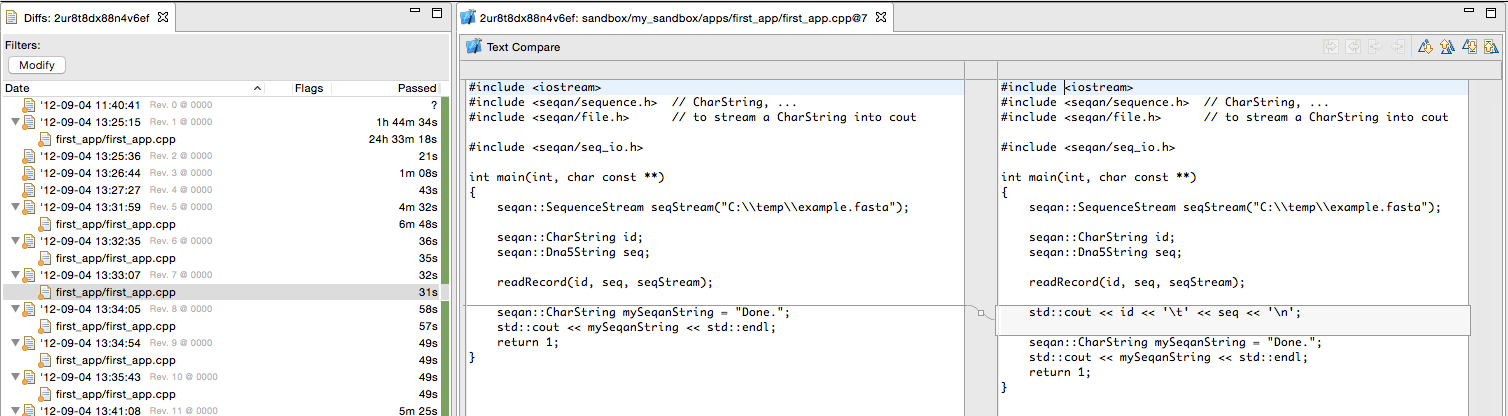
\includegraphics[width=1.0\linewidth]{Figures/AnalysisDiff.png}
  \caption[Beispielhafte Diff-Datei]{Dieser \gls{apiua}-Bildschirmausschnitt zeigt den Probanden \texttt{2ur8t8dx88n4v6ef}. Zu sehen sind im linken Drittel die ID des Probanden (im Tab), seine Kompilierversuche (Knoten erster Ordnung), alle bearbeiteten Dateien (Kindknoten), deren Kompiliererfolg (grüne, gelbe oder rote Icon-Annotation) und die auf sie verwendete Zeit. \\Im rechten Teil des Ausschnitts kann man die aktuell betrachtete Datei vollständig in ihrem vorangegangenen und aktuellen Zustand sehen. Die Codeänderungen sind grafisch hervorgehoben.}
  \label{fig:AnalysisDiff}
\end{figure}



\subsection{Beispiel: Doclog-Datei}
\label{sec:doclog}

Eine Doclog\footnote{\textbf{doc}umentation \textbf{log}}-Datei dokumentiert alle Zugriffe/Ereignisse auf die, im Internet bereitgestellte SeqAn-Dokumentation. Diese Dokumentation besteht hauptsächlich aus der Dokumentation selbst und den Tutorials.

Die Erfassung der Dokumentationszugriffe soll schwer nachvollziehbare Entwicklungsschritte zwischen zwei Kompilierversuchen vereinfachen. So können größere Code-Einfügungen bedeuten, dass dem Probanden ein Licht aufgegangen ist. Sie können aber auch bedeuten, dass der eingefügte Code schlicht von der Online-Dokumentation kopiert wurde. Letztere Interpretation kann aber nur zuverlässig vollzogen werden, wenn man dafür triftige Indizien hat. 

\begin{center}
\usemintedstyle{bw}
\begin{minted}[linenos=true,firstnumber=481]{sh}
2012-09-04T14:14:23.729+02:00 READY http://trac.seqan.de/wiki/Tutorial/ GettingStarted 160.45.233.238 - 0 0 1350 612
2012-09-04T14:14:26.774+02:00 SCROLL http://trac.seqan.de/wiki/Tutorial/ GettingStarted 160.45.233.238 - 0 228 1350 612
2012-09-04T14:14:27.463+02:00 LINK-http://trac.seqan.de/wiki/Tutorial/ GettingStarted/WindowsVisualStudio http://trac.seqan.de/wiki/Tutorial/ GettingStarted 160.45.233.238 - 0 228 1350 612
2012-09-04T14:14:27.784+02:00 UNLOAD http://trac.seqan.de/wiki/Tutorial/ GettingStarted 160.45.233.238 - 0 228 1350 612
2012-09-04T14:14:28.804+02:00 READY http://trac.seqan.de/wiki/Tutorial/ GettingStarted/WindowsVisualStudio 160.45.233.238 - 0 147 1350 612
2012-09-04T14:14:35.196+02:00 SCROLL http://trac.seqan.de/wiki/Tutorial/ GettingStarted/WindowsVisualStudio 160.45.233.238 - 0 3420 1350 612
2012-09-04T14:14:49.711+02:00 SCROLL http://trac.seqan.de/wiki/Tutorial/ GettingStarted/WindowsVisualStudio 160.45.233.238 - 0 4104 1350 612
2012-09-04T14:14:53.414+02:00 SCROLL http://trac.seqan.de/wiki/Tutorial/ GettingStarted/WindowsVisualStudio 160.45.233.238 - 0 3876 1350 612
2012-09-04T14:15:00.302+02:00 SCROLL http://trac.seqan.de/wiki/Tutorial/ GettingStarted/WindowsVisualStudio 160.45.233.238 - 0 3648 1350 612
2012-09-04T14:15:06.149+02:00 BLUR http://trac.seqan.de/wiki/Tutorial/ GettingStarted/WindowsVisualStudio 160.45.233.238 - 0 3648 1350 612
2012-09-04T14:15:21.071+02:00 FOCUS http://trac.seqan.de/wiki/Tutorial/ GettingStarted/WindowsVisualStudio 160.45.233.238 - 0 3648 1350 612
\end{minted}
\captionof{listing}[Beispiel: Auszug aus einer Doclog-Datei]{Auszug aus einer Doclog-Datei}
\label{lst:doclog-file}
\end{center}

Die Doclog-Datei ist eine Tabulator-separierte Liste. Ihre Spalten sind:

\begin{description}
	\item[DateTime] Zeitstempel in ISO8601
	\item[Action] Ereignis (READY, UNLOAD, FOCUS, LINK, SCROLL, etc.)
	\item[URI] Adresse der geöffneten Seite
	\item[IP] IP des Anwenders
	\item[ProxyIP] Proxy-IP des vom Anwender verwendeten HTTP-Proxies
	\item[ScrollX] Scrollposition X-Achse in Pixeln (px) vom oberen Rand des Dokuments
	\item[ScrollY] Scrollposition Y-Achse in Pixeln (px) vom linken Rand des Dokuments
	\item[Width] Breite des Browser-Ansichtsbereichs (Viewport) in Pixeln (px)
	\item[Height] Höhe des Browser-Ansichtsbereichs (Viewport) in Pixeln (px)
\end{description}

Die in der Doclog-Datei dokumentierte Nutzung der Online-Dokumentation durch den Probanden zeigt also, dass er das Tutorial \textit{Getting Started} um 14:14 Uhr öffnete (Zeile 1) und anschließend vertikal um 228px nach unten scrollte (Zeile 2). Zeile 3 zeigt, dass er den Link auf die SeqAn-Installationsanleitung für Visual Studio öffnete und dabei die, eben noch geöffnete Seite schloss (Zeile 4). Anschließend gab es mehrere Scrollaktionen auf der eben geöffneten Seite. In Zeile 10 verlor die Seite den Fokus, um ihn in Zeile 11, etwa 15s später, wiederzuerlangen.

Mit ein wenig Übung kann man das Protokoll gut lesen, allerdings kaum gewinnbringend verwenden. Die Daten wurden dokumentiert, um den Gedankengang des Probanden bei seiner Arbeit zwischen zwei Kompilierversuchen besser nachvollziehen zu können. Die Zeitstempel der Kompilierversuche und die der Aktionen auf der Online-Dokumentation müssen also verknüpft werden. Darüber hinaus ist noch nichts darüber gesagt, was genau der Anwender auf der Online-Dokumentation gesehen hat. Dazu müsste man selbst die Dokumentation öffnen, die Größe des Browsers korrekt anpassen und an dieselbe Position scrollen. Spätestens, wenn eine Dokumentationsseite durch einen SeqAn-Entwickler verändert wurde, lässt sich die Information nicht oder nur unverhältnismäßig aufwändig wiederbeschaffen.

In APIUA muss nicht das Rohformat vom Forscher analysiert werden, sondern dessen Aufbereitung. Dazu werden intern, für noch nicht prozessierte Doclog-Einträge, Browser-Instanzen erzeugt, die die jeweilige URI laden, den Anzeigebereich auf die korrekte Größe setzen, an die dokumentierte Scrollposition springen, eventuelle Texteingaben vornehmen und einen Screenshot erzeugen. Diese können dann bei der Analyse von Diff-Dateien zu Rate gezogen werden. \autoref{fig:AnalysisDoclog} zeigt eine geöffnete Datei mit einem schwebenden Fenster in der rechten Bildschirmhälfte, das den Screenshot für die, in diesem Moment vom Probanden geöffneten Seite zeigt.

\begin{figure}
  \centering
    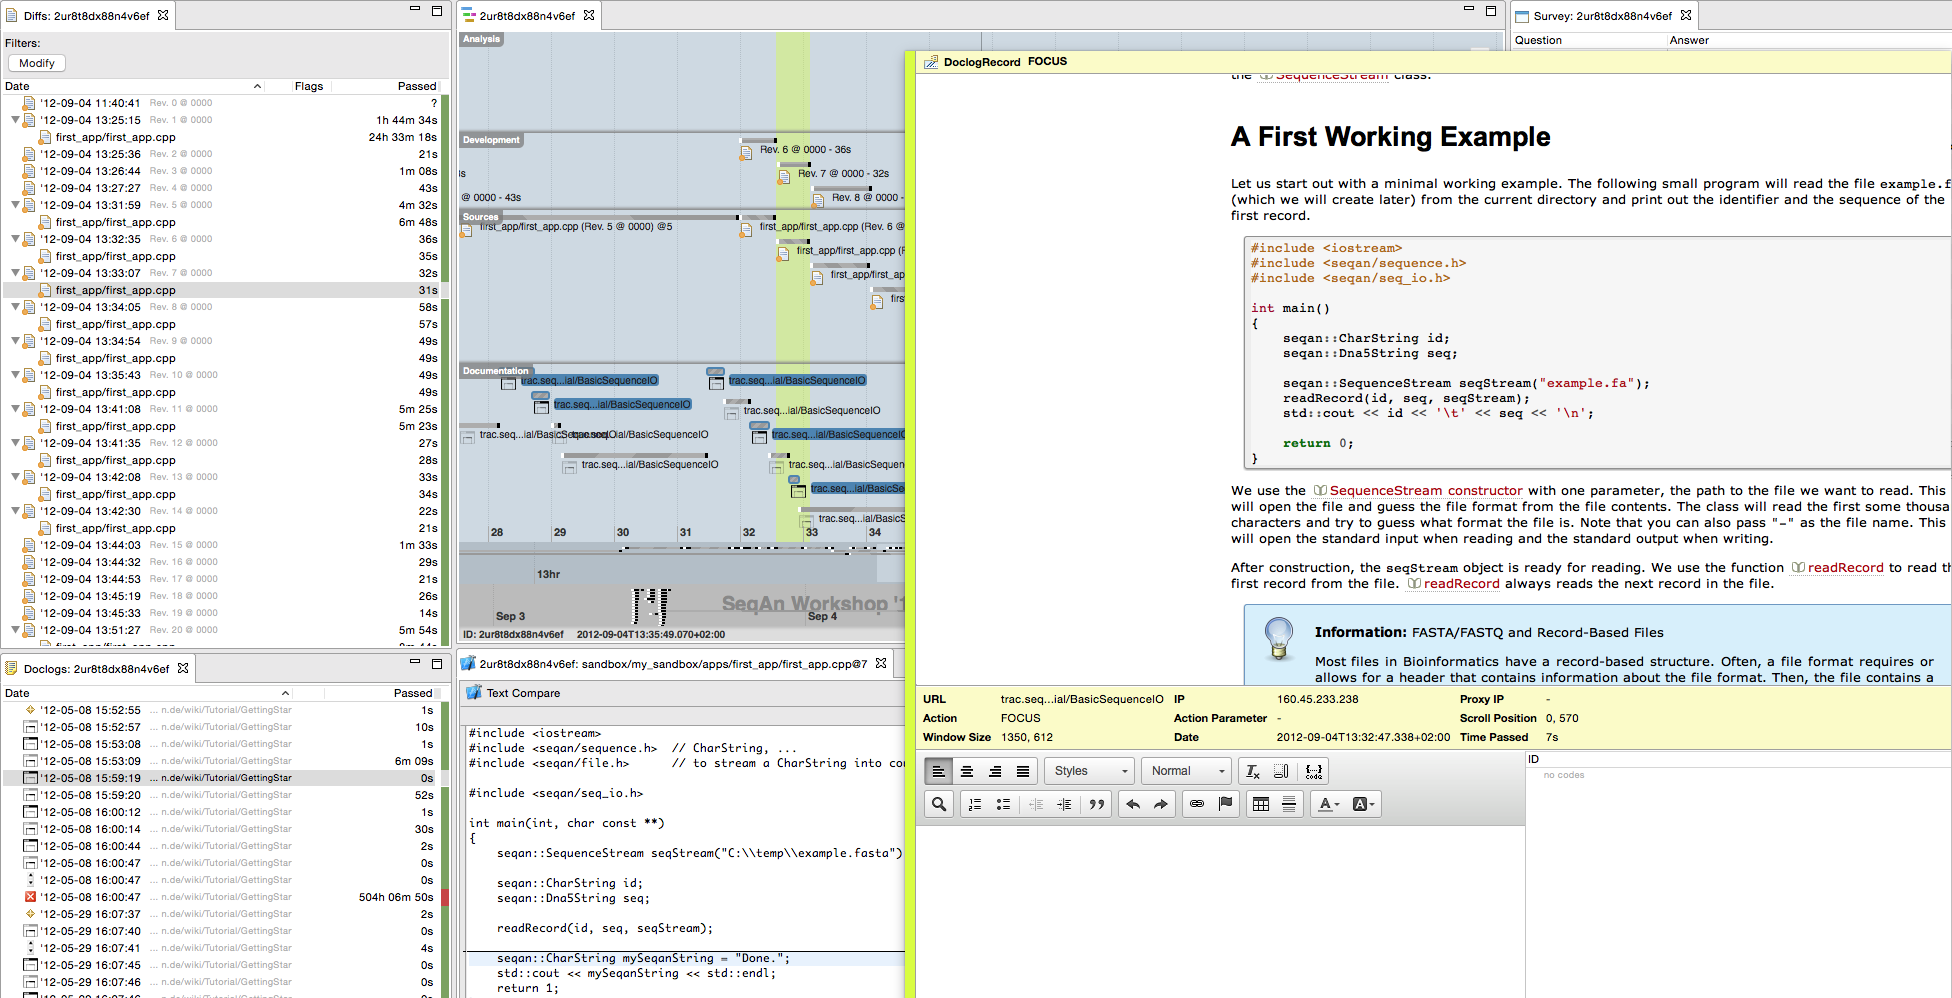
\includegraphics[width=1.0\linewidth]{Figures/AnalysisDoclog.png}
  \caption[Beispielhafte Doclog-Datei]{Dieser \gls{apiua}-Bildschirmausschnitt zeigt den Probanden \texttt{2ur8t8dx88n4v6ef}. Die Beschreibung des linken Bildbereichs kann \autoref{fig:AnalysisDiff} entnommen werden. Der blaue Bereich in der Mitte zeigt einen Abschnitt der Zeitleiste, auf der sich sämtliche Datenpunkte zum Probanden befinden. In Neon ist die Zeitspanne hervorgehoben, die zwischen dem vergangenen und dem aktuellen Kompilierversuch liegt. In der rechten Hälfte ist ein schwebender Dialog dargestellt, der Informationen zu dem Element darstellt, über dem gerade die Maus schwebt. Konkret handelt es sich um einen Doclog-Eintrag bestehend aus dem Screenshot, darunter den Metainformationen und der (leeren) Memo.}
  \label{fig:AnalysisDoclog}
\end{figure}



\subsection{Herausforderungen für ein GTM-Datenanalysewerkzeug}

Die beiden Beispiele sollten zeigen, dass \begin{enumerate}
\itemsep1pt\parskip0pt\parsep0pt
  \item hochstrukturierte Daten viele Informationen enthalten,
  \item die teilweise nur sehr aufwändig und
  \item fehleranfällig extrahiert werden können und
  \item damit potentiell die Sorgfalt bei der Anwendung der \gls{gtm} schmälert.
\end{enumerate}

Die Aufgabe eines \gls{gtm}-Datenanalysewerkzeugs darf also nicht nur darin bestehen, die Analyse technisch irgendwie zu ermöglichen. Sie besteht auch darin, zeitraubende und fehlerträchtige Routinearbeiten adäquat zu automatisieren und die Phasen und Praktiken der \gls{gtm} reibungslos zu erlauben. Die durch die \gls{gtm} ohnehin schon stark geforderte Sorgfalt und Disziplin des Forschers, dürfen durch das Datenanalysewerkzeug nicht unnötig strapaziert werden, da sonst die Qualität der generierten \gls{gt} gefährdet wäre.

Als Forscher, der sich selbst in die \gls{gtm} einarbeitete, sogar das für die eigene Datenanalyse zugehörige Analysewerkzeug selbst entwickelte und im ständigen Austausch mit seiner \gls{gtm}-affinen Forschungsgruppe\footnote{Allein diese Ausrichtung scheint äußerst selten zu sein. Zumindest wenn man sich eine Stichprobe der in führenden Softwaretechnik-Zeitschriften der Jahre 1995-1999 veröffentlichten Artikel ansieht: Demnach wurde die \gls{gtm} in weniger als 1\% der Arbeiten verwendet. \citep{Glass:2002ec}} stand, konnte ich eine Reihe von, in \autoref{tab:APIUARequirements} zusammengefassten Anforderungen formulieren.

\begin{landscape}
\begin{longtable}{p{0.2\linewidth} p{0.35\linewidth} p{0.35\linewidth}}  
  \multicolumn{1}{l}{\textbf{Anforderung}} & \multicolumn{1}{l}{\textbf{Beschreibung}} & \multicolumn{1}{l}{\textbf{Erfüllung durch \gls{apiua}}} \\ \hline 
  \endfirsthead

  \multicolumn{3}{c}{\tablename\ \thetable{} -- \textit{Fortsetzung}} \\
  \multicolumn{1}{l}{\textbf{Anforderung}} & \multicolumn{1}{l}{\textbf{Beschreibung}} & \multicolumn{1}{l}{\textbf{Erfüllung durch \gls{apiua}}} \\ \hline 
  \endhead

  \\
  \multicolumn{3}{r}{\textit{Fortsetzung auf nächster Seite}} \\
  \endfoot

  \caption{Anforderungen an \gls{gtm}-Datenanalysewerkzeuge}
  \label{tab:APIUARequirements} \\
  \endlastfoot

  Große Datenmengen &
  Die Verarbeitung von mehreren Gigabyte Datenmaterial muss unterstützt sein. &
  Auf einem durchschnittlichen Computer konnten 24GB Datenmaterial verarbeitet werden. \\
  
  Datenformate &
  Videos, Audioaufnahmen, Textdokumente, aber auch etablierte Datenaustauschformate wie XML und JSON müssen unterstützt werden. Die unterstützten Datenformate müssen erweiterbar sein. &
  Unterstützt werden lediglich die im Rahmen dieser Arbeit erfassten Datenformate. Ein \gls{plugin}-Mechanismus erlaubt die Erweiterung um beliebige weitere Datenformate (siehe \autoref{fig:apiua-plugins}). \\
  
  Offenes Kodieren &
  Die Phase des offenen Kodierens muss optimal (Kategorien, Eigenschaften, etc.) unterstützt werden. &
  Offenes Kodieren wird umfänglich unterstützt (siehe \autoref{fig:apiua-opencoding-cd}). Kategorien werden in Form von Kode-Hierarchien ermöglicht (siehe \autoref{fig:apiua-codes}). Eigenschaften werden auf Kode-Ebene definiert; entsprechende Wertebelegungen auf Kodeinstanz-Ebene erlaubt (siehe \autoref{fig:apiua-properties}). \\
  
  Axiales Kodieren &
  Die Phase des axialen Kodierens muss optimal (Relationen, etc.) unterstützt werden. Es muss Funktionen geben, die dabei helfen, \glspl{acm} zu abstrahieren. &
  Axiales Kodieren wird umfänglich unterstützt. Relationen werden auf Kode-Ebene definiert und können verankert werden. Aus den vorhandenen Relationen können automatisch \glspl{ac} und \glspl{acm} erzeugt werden (siehe \autoref{fig:apiua-axialcoding}). Abstrahierungsfunktionen existieren rudimentär in Form fest implementierter Interferenzregeln. \\
  
  Selektives Kodieren &
  Die Phase des selektiven Kodierens muss stark unterstützt werden. Dazu werden Funktionen benötigt, welche die eine weiter gehende Abstraktion / Generalisierung von Kodes, Relationen und schließlich von \glslink{acm}{axialen Kodiermodellen} erlauben. &
  Selektives Kodieren wird teilweise durch \gls{apiua}s Interferenzmöglichkeiten und Verallgemeinerung- und Zusammenfassungsmöglichkeiten von Relationen unterstützt. \\
  
  Implizites Wissen &
  In den von dem Anwender gefunden Verankerungen verbirgt sich in manchen Fällen implizites Wissen. Das Werkzeug sollte derartiges Wissen sichtbar machen. Weitere Details siehe weiter unten. &
  Implizite Verankerungen und Relationen werden sichtbar gemacht. \\
  
  Vorwissen &
  Es muss die Möglichkeit geben Verankerungen, die auf Vorwissen des Forschers beruhen, vorzunehmen. &
  Vorwissen kann durch die Verwendung von \url{bibtex:}- und \url{file:}-\acrshort{uri}s verankert werden. \\
  
  Umstrukturierungs-\\operationen\footnote{Auch wenn man verführt ist, die Bezeichnung \textit{Refactoring} zu verwenden, wäre die von \cite{Fowler:424198} formulierte Anforderung verletzt, dass die Semantik bei einer derartigen Operation nicht verändert wird. Eine kanonische Übertragung dieser Eigenschaft auf Theorien ist nicht möglich, da die Grenzen einer Theorie nicht hinreichend scharf sind. Während man sich noch streiten kann, ob einfache Operationen, wie eine Kode-Umbenennung, bereits die Semantik einer Theorie ändern, ist die Frage bei komplexeren Operationen wie die Verallgemeinerung von Relationen eindeutig mit ``ja'' zu beantworten.} &
  Es muss Möglichkeiten geben, Änderungen an der Modellierung vorzunehmen, die der \gls{gt} zu Grunde liegt. Beispiele sind Kode-Umbenennung, Verallgemeinerung oder Spezialisierung von Relationen, Verschieben von Kode-Eigenschaften und Zusammenfassung oder Auftrennen von Kodes. &
  Einige Strukturänderungsoperationen werden unterstützt. Dazu gehören einfache Operationen wie die Umordnung des Kode-Baumes und die Verallgemeinerungen bzw. Zusammenfassung von Relationen (siehe \fref{fig:apiua-feature-generalization-relation}). Außerdem können während der Zuweisung von Phänomenen zu Kodes in einem speziellen Dialog (siehe \fref{fig:apiua-feature-properties-assignment}) direkt Eigenschaftswerte zugewiesen werden. \\
  
  Weitergehende Analysefunktionen &
  Beispielsweise könnte eine Funktion, die anzeigt, welche Kodes in welchen Datenquellen/-erhebungen verankert sind, bei der Bewertung der Frage helfen, ob und in welche Richtung eine weitere Datenerhebung gehen kann/soll. Diese Funktion würde also den Forscher beim \textit{theoretischen Sampling} unterstützen. &
  Weitere Analysefunktionen wurden aus zeitlichen Gründen nicht implementiert. \\
  
  Interoperabilität &
  Die Forschungsergebnisse müssen in einem Format gespeichert werden, das sich zur Weiterverarbeitung durch dritte Programme eignet. Darüber hinaus erlaubt die Verwendung standardisierter Datenformate die Bereitstellung der Forschungsdaten im Rahmen von \textit{Open Science} --- also in diesem Fall, dem freien Zugang zu wissenschaftlichen Ergebnissen. &
  Die Forschungsergebnisse werden in XML abgelegt. Memos werden in Form von HTML-Dateien abgelegt, deren Name der \gls{uri} des beschriebenen Datenpunktes entspricht. \Glspl{acm} liegen in Form von JSON-Dateien vor. Datenpunkte werden innerhalb der HTML- und JSON-Dateien einheitlich mit deren \gls{uri} referenziert, was jede Möglichkeit von technischer Datenredundanz ausschließt.  \\
  
  Usability &
  Die Usability des Werkzeugs selbst muss hoch sein, um die Qualität der erarbeiteten \gls{gt} nicht zu schmälern. &
  Der Zustand der Arbeitsumgebung wird vollständig gesichert, d.h. die Anordnung der verschiedenen Bereiche, deren Anzeigeoptionen, deren Inhalt und viele weitere Informationen, wie zuletzt verwendete Kodes, werden nach einem Neustart der Anwendung wiederhergestellt. Zur Erfüllung einer Aufgabe werden verschiedene Möglichkeiten angeboten. Zuletzt verwendete Elemente (Kodes, Phänomene, etc.) werden in einer Historie festgehalten. Kodes werden automatisch mit sinnvollen Farben versehen. \\
  
  Plattformabhängigkeit & --- & \gls{apiua} ist lauffähig unter Windows, Mac OS und Linux.\\
\end{longtable}
\end{landscape}

\begin{figure}
  \centering
    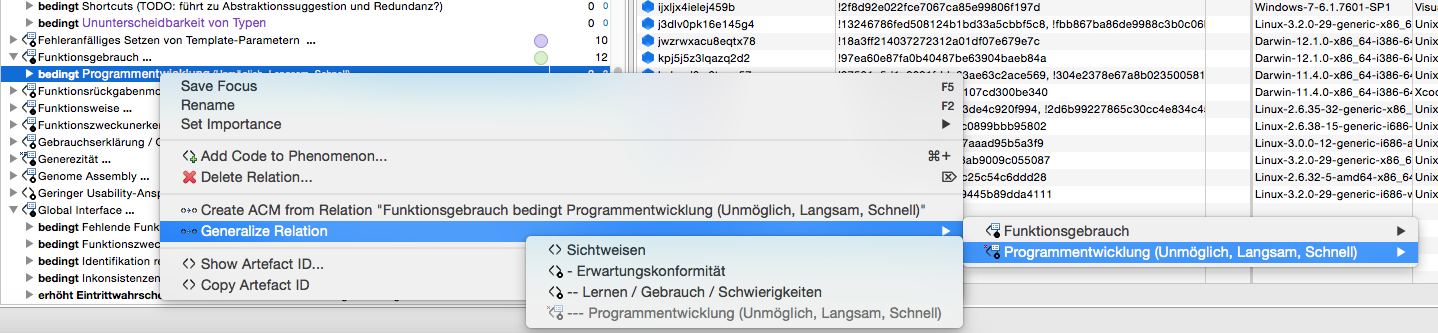
\includegraphics[width=1.0\linewidth]{Figures/apiua/feature-generalization-relation.png}
  \caption[APIUA: Verallgemeinerung von Relationen]{Dieser Screenshot von \gls{apiua} zeigt das die Möglichkeit zur Verallgemeinerung von Relationen.}
  \label{fig:apiua-feature-generalization-relation}
\end{figure}

\begin{figure}
  \centering
    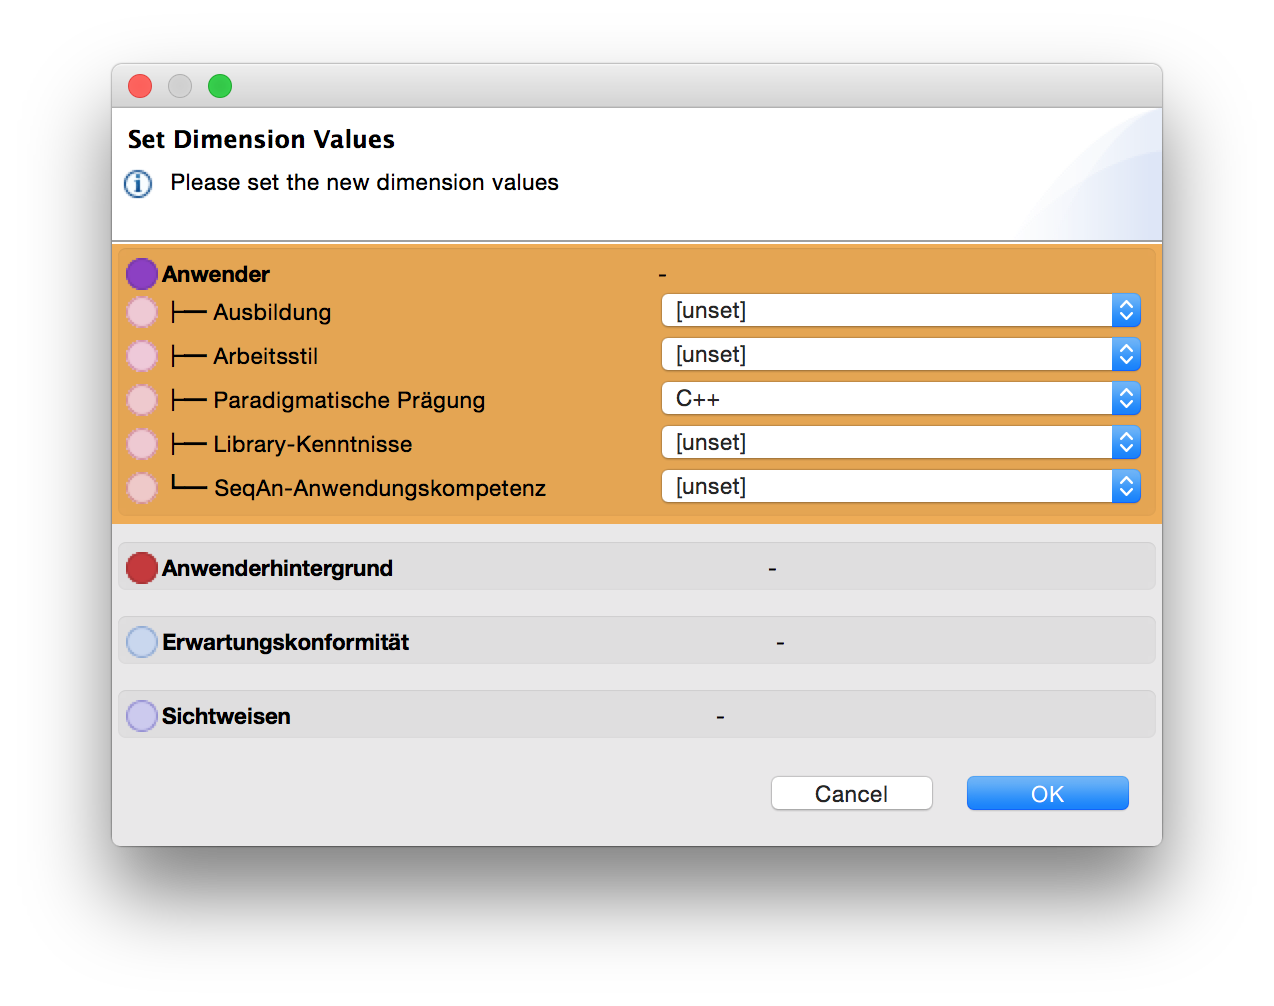
\includegraphics[width=0.5\linewidth]{Figures/apiua/feature-properties-assignment.png}
  \caption[APIUA: Wertezuweisung bei Umstrukturierungen]{Dieser Screenshot von \gls{apiua} zeigt den Dialog zur Zuweisung von Eigenschaftswerten bei Umstrukturierungen.}
  \label{fig:apiua-feature-properties-assignment}
\end{figure}

Im \sref{sec:gtm-implementation} auf Seite \pageref{sec:gtm-implementation} gehe ich genauer auf einige der Anforderungen und ihrer Erfüllung durch \gls{apiua} ein. Der folgende Abschnitt soll zunächst den groben technischen Aufbau von \gls{apiua} vorstellen.

\begin{figure}
  \centering
    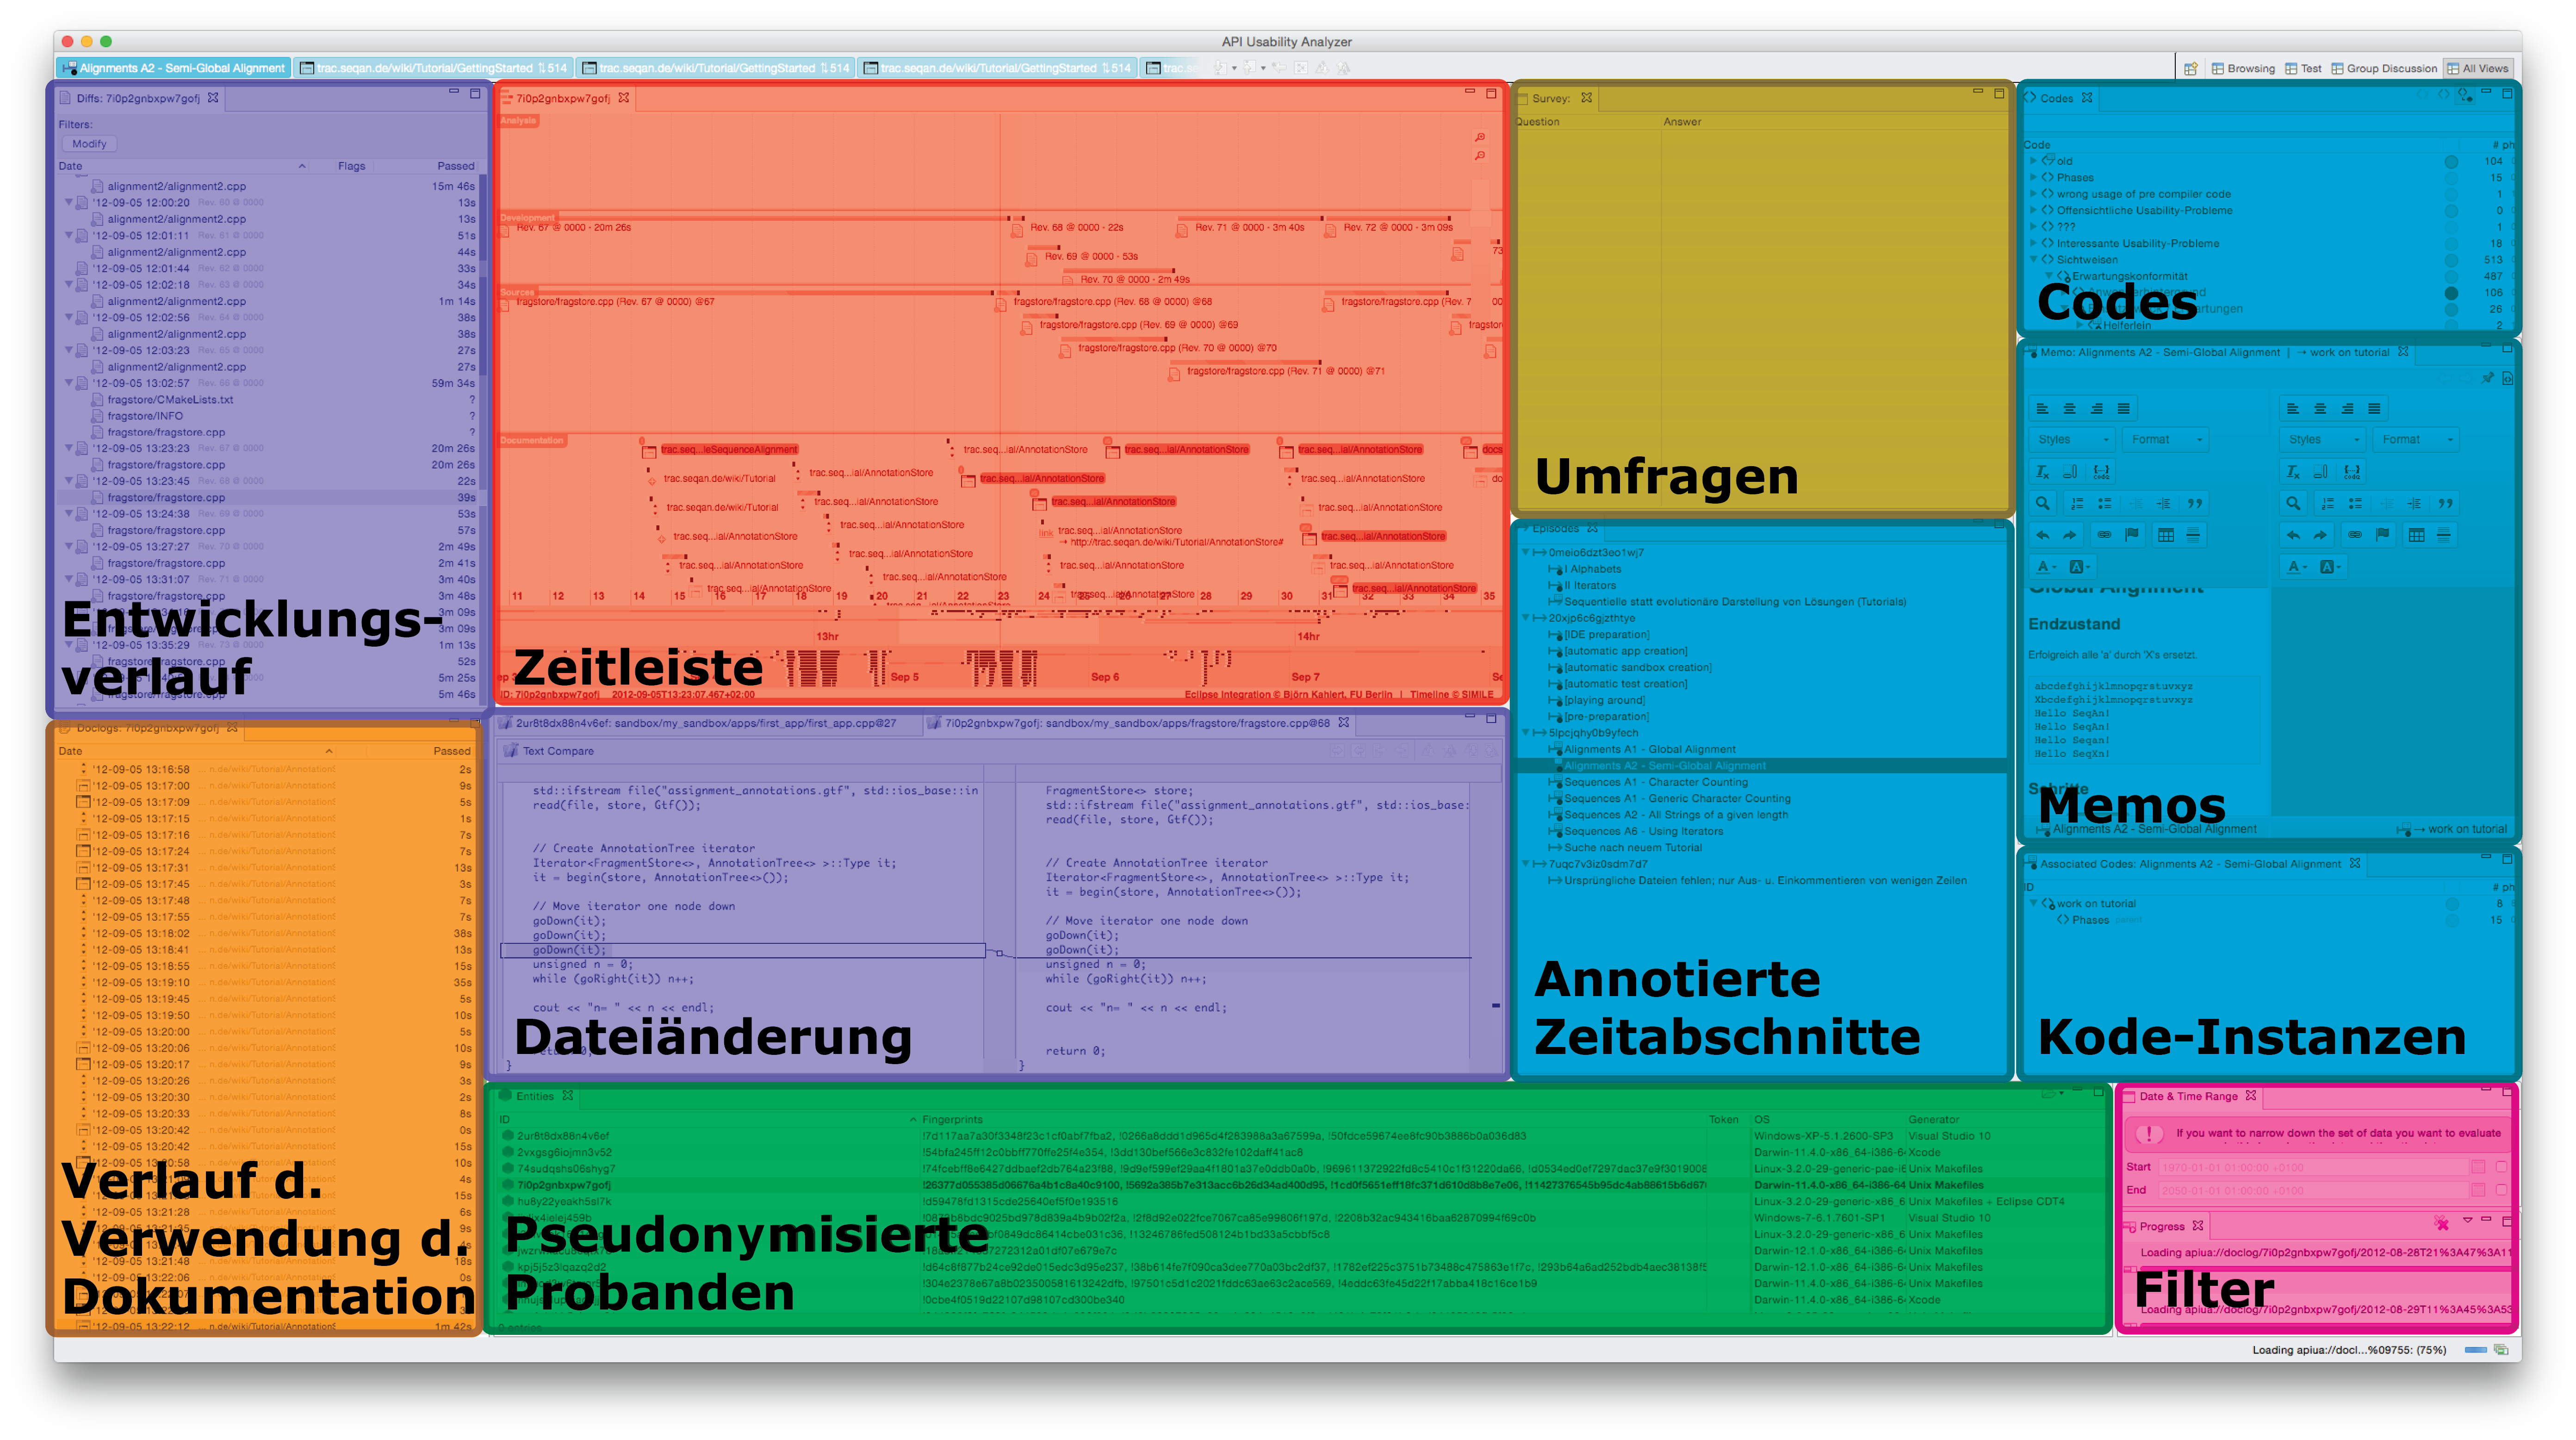
\includegraphics[width=1.0\linewidth]{Figures/apiua/plugins.png}
  \caption[APIUA: Architektur --- Plugins]{Dieser Screenshot von \gls{apiua} in der Perspektive für offenes Kodieren zeigt die von den verschiedenen \glspl{plugin} der Schicht 3 beigesteuerten Eclipse-Views.\\
  V.\,l.\,n.\,r.: Violett: Diff-\gls{plugin}; Rot: Timeline-\gls{plugin}; Gelb: Stats-\gls{plugin}; Blau: GTM-\gls{plugin}; Orange: Doclog-\gls{plugin}; Grün: Entity-\gls{plugin}; Pink: Core-\gls{plugin}}
  \label{fig:apiua-plugins}
\end{figure}

\begin{figure}
  \centering
    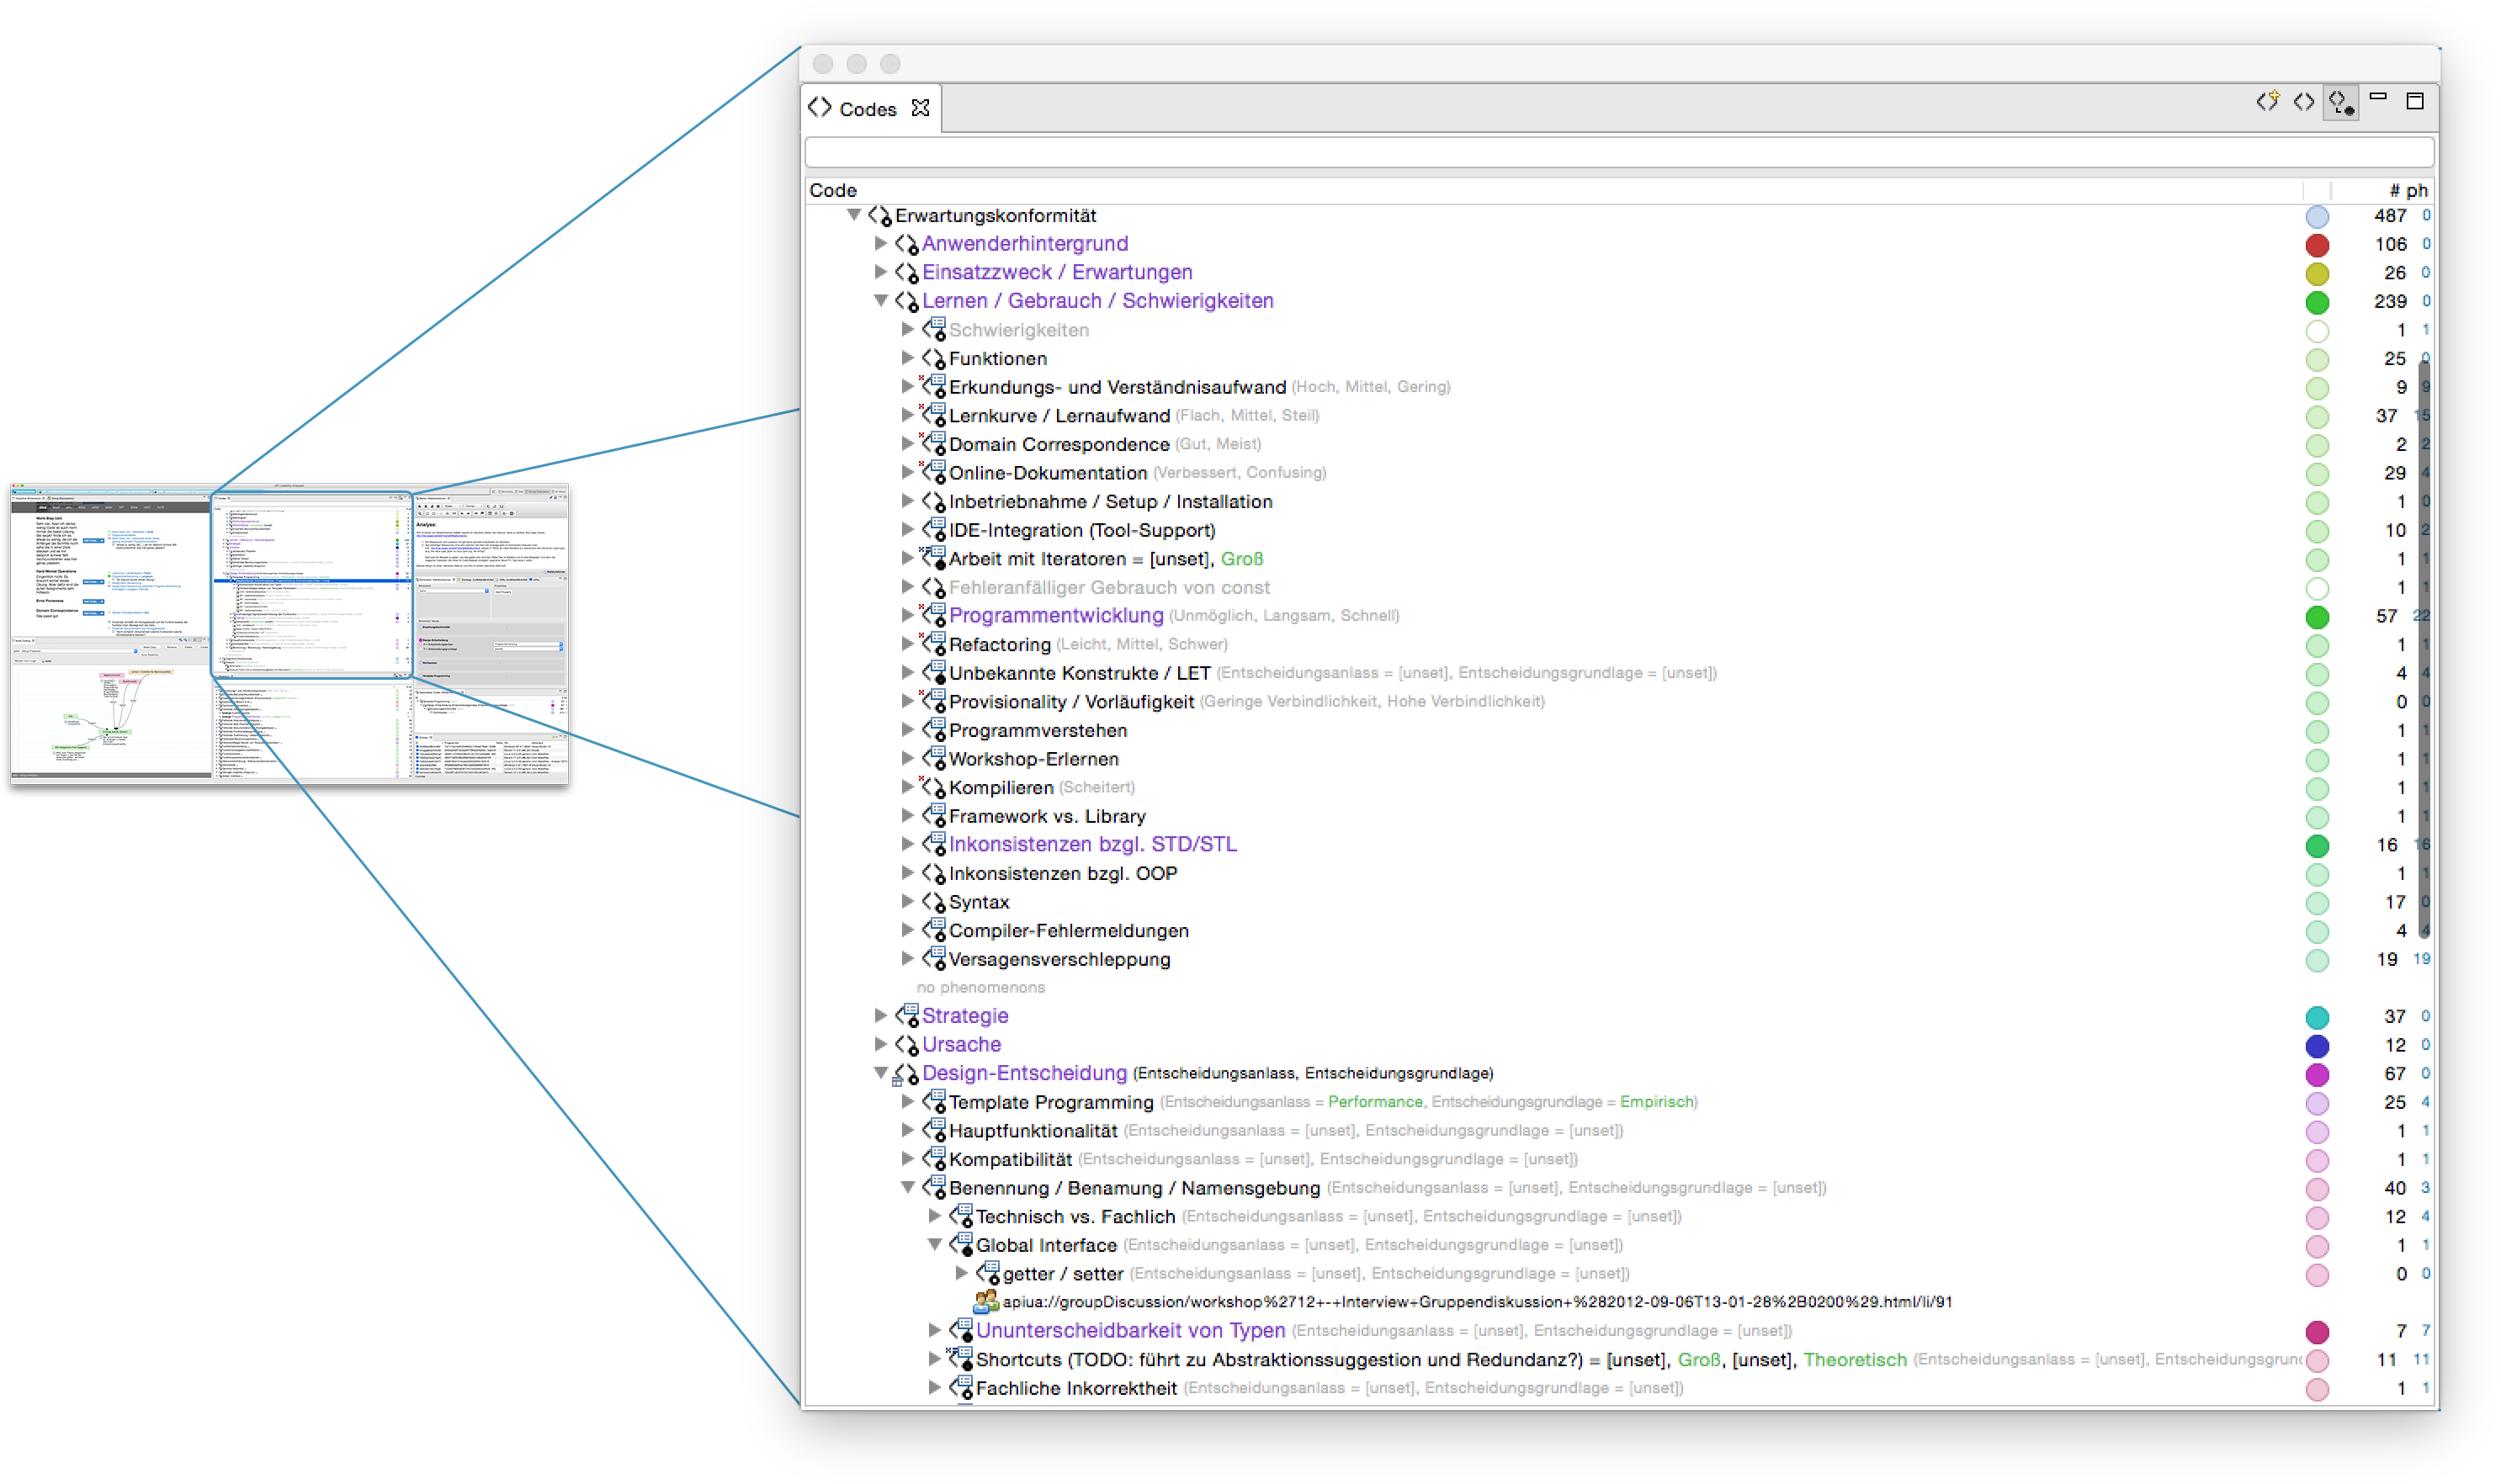
\includegraphics[width=1.0\linewidth]{Figures/apiua/codes.png}
  \caption[APIUA: Kode-Ansicht]{Dieser Screenshot von \gls{apiua} zeigt das Eclipse-View ``Codes'', das alle verankerten Kodes darstellt.}
  \label{fig:apiua-codes}
\end{figure}

\begin{figure}
  \centering
    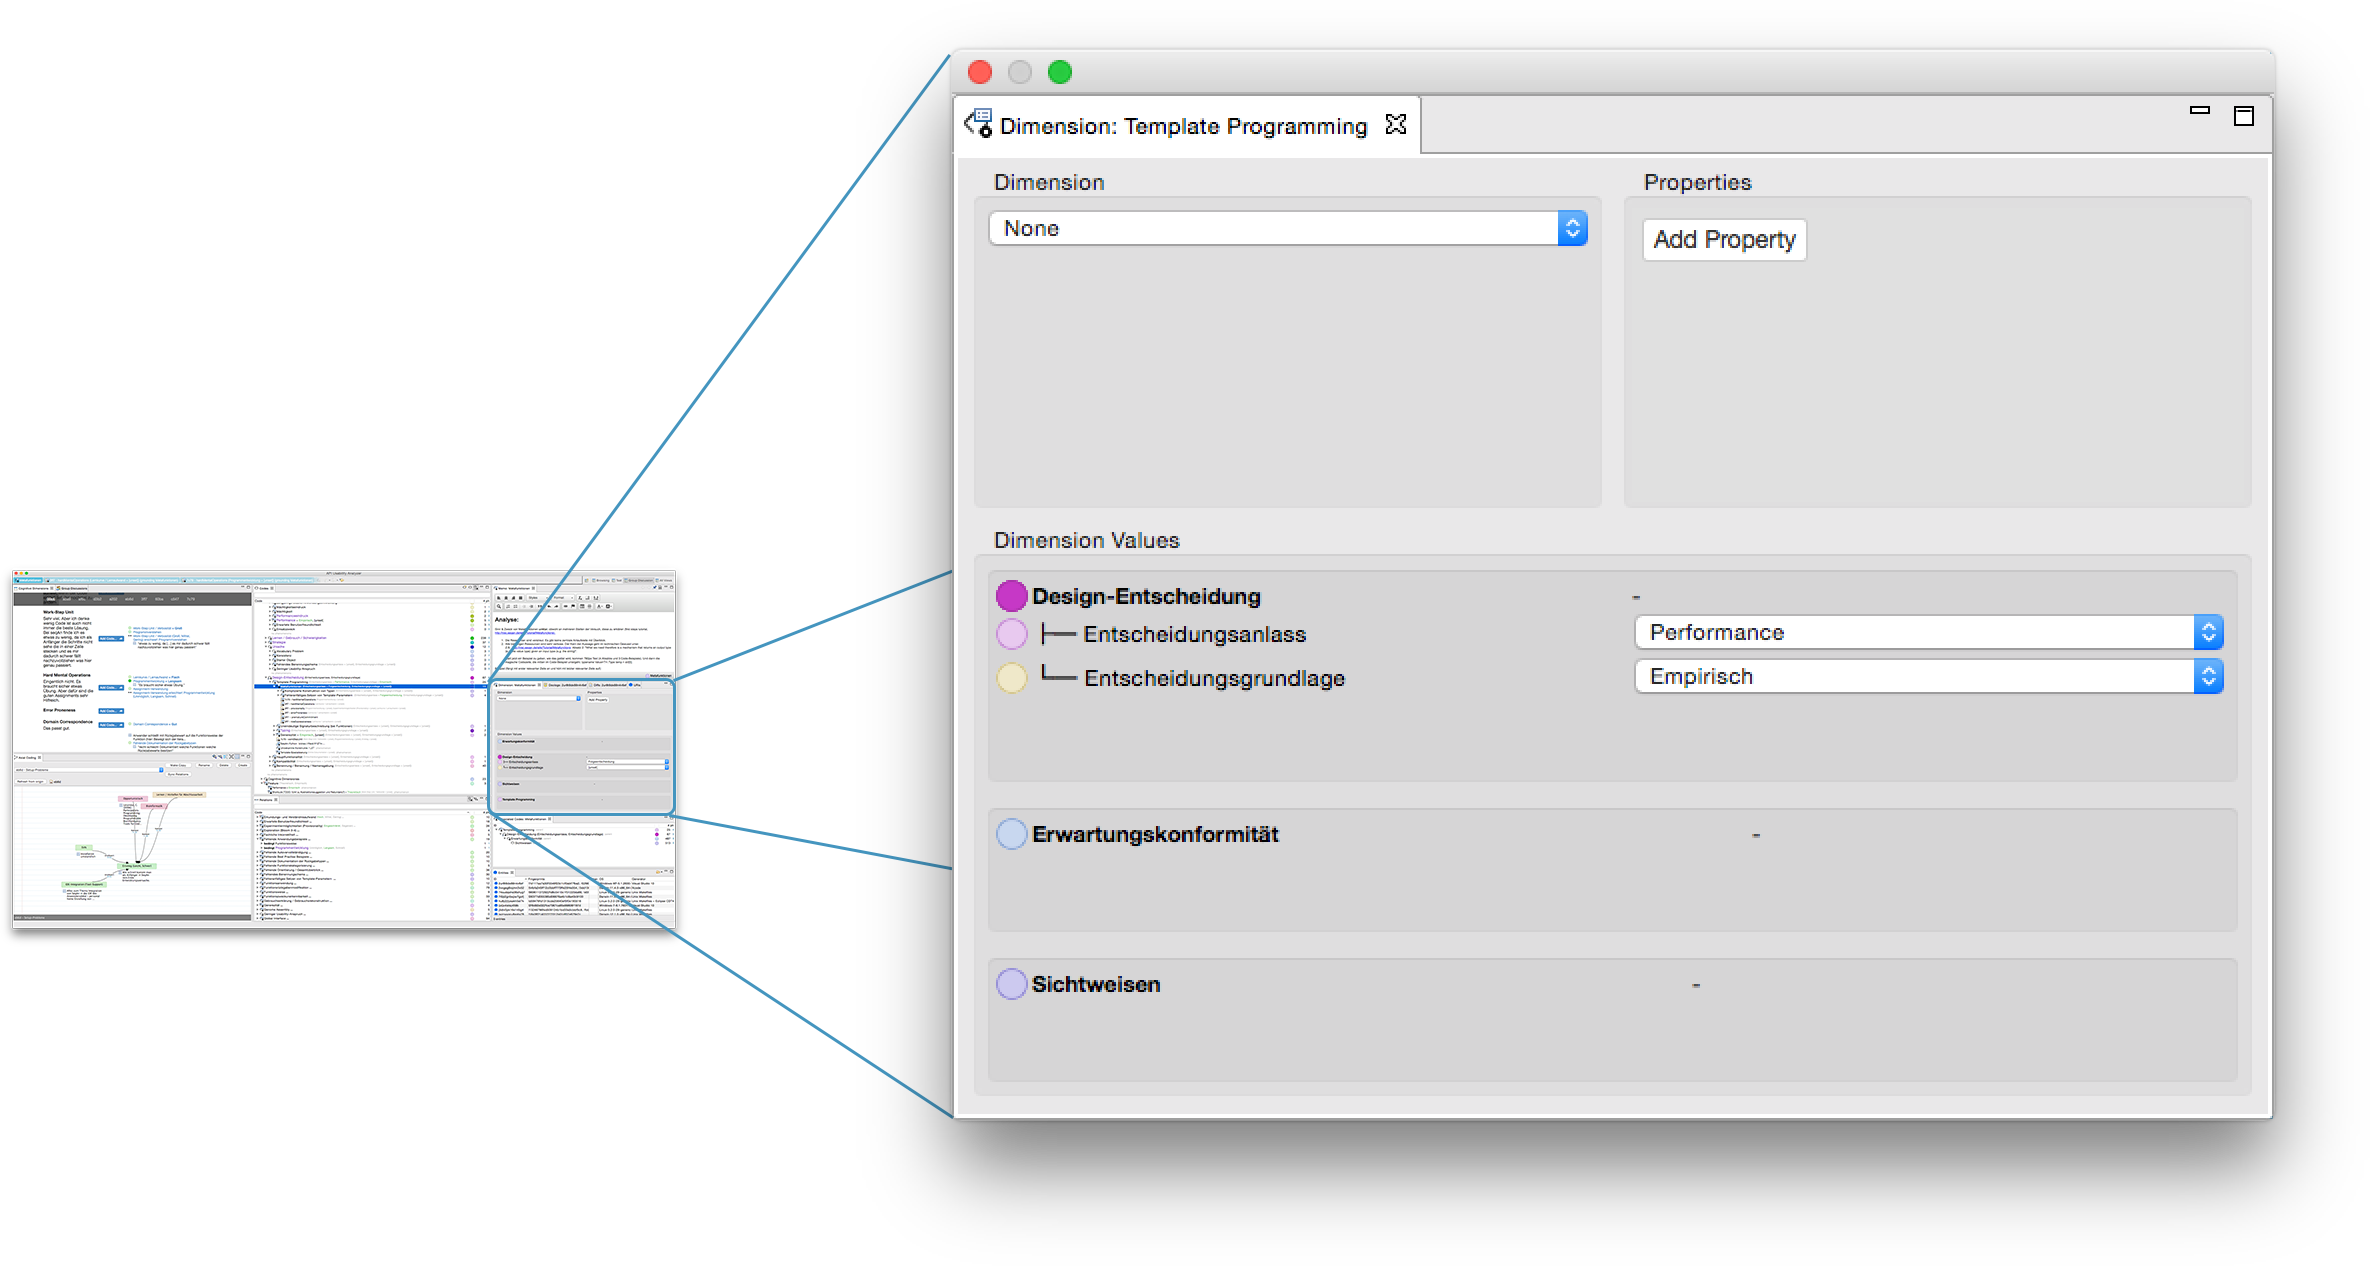
\includegraphics[width=1.0\linewidth]{Figures/apiua/properties.png}
  \caption[APIUA: Eigenschaften-Ansicht]{Dieser Screenshot von \gls{apiua} zeigt das Eclipse-View ``Dimension'', das die Dimension, alle Eigenschaften und Wertebelegungen für das aktuell selektierte Element darstellt.}
  \label{fig:apiua-properties}
\end{figure}



\subsection{Entwurf}

In diesem Abschnitt werden die wichtigsten \gls{apiua}-Entwurfsentscheidungen vorgestellt. Die vollständigen Quellen von \gls{apiua} sind unter \gls{github}\footnote{\url{https://github.com}} veröffentlicht und werden dort gepflegt.

\Gls{apiua} basiert auf der \textit{\gls{rcp}}\footnote{\url{http://wiki.eclipse.org/index.php/Rich\_Client\_Platform}} (Version 3), die wiederum die Grundlage für die bekannte Entwicklungsumgebung \textit{\gls{eclipse}} darstellt.

Architektonisch verwendet \gls{apiua} einen Hybrid aus einer serviceorientierten und einer schichtenbasierten Architektur (siehe \autoref{fig:Architecture}).

\begin{figure}
  \centering
    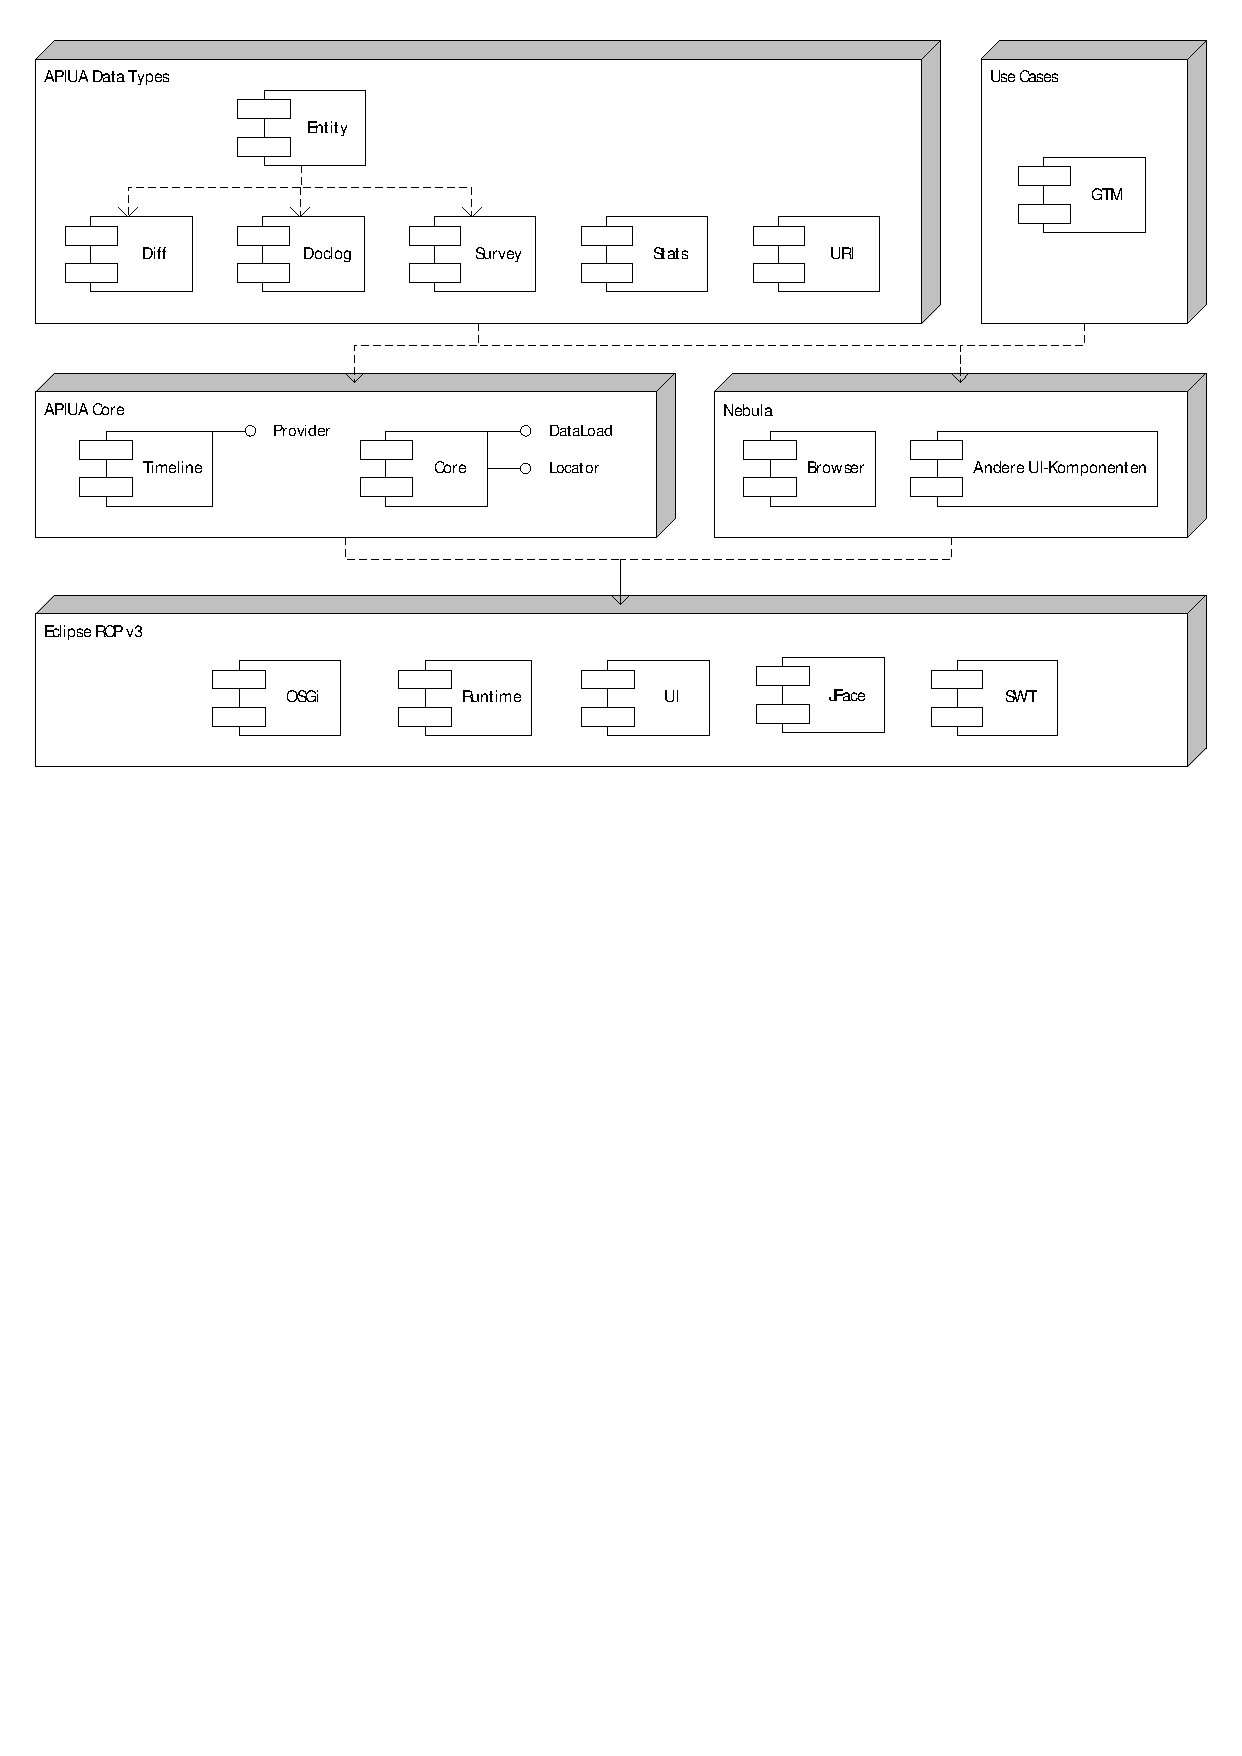
\includegraphics[width=1.0\linewidth,trim=0cm 16.5cm 0cm 0cm]{Figures/architecture.pdf}
  \caption[APIUA: Architektur --- Schichten]{Dieses UML-Diagramm beschreibt die Architektur von \gls{apiua}. Sie besteht aus den folgenden drei Schichten: \gls{rcp}-Schicht, Infrastrukturerweiterungsschicht (Core und Nebula),  Komponentenschicht (Data Types, Use Cases).}
  \label{fig:Architecture}
\end{figure}


\subsubsection{Schicht 1: Eclipse Rich Client Platform}

Die unterste Schicht bildet die \gls{rcp}-Schicht und stellt das Fundament von \gls{apiua} dar.

Die Komponenten \textit{\acrshort{osgi}} und \textit{Runtime} stellen den, von \gls{eclipse} bekannten Plugin-Mechanismus bereit und erlauben es, die Kopplung zwischen Modulen (hier: \gls{plugin}s) erheblich zu verringern. Die \textit{\gls{swt}}-Komponente erlaubt den plattformübergreifend einheitlichen Zugriff auf plattformabhängige UI-Elemente. \textit{JFace} und \textit{UI} ermöglichen die, von \gls{eclipse} bekannte, Organisation des Anwendungsfensters mit Hilfe von Perspektiven, Editoren und Ansichten (engl. \textit{views}).


\subsubsection{Schicht 2: Infrastrukturerweiterung}

Die zweite Schicht besteht aus zwei Teilen, die die \gls{rcp}-Schicht um weitere Infrastruktur-Funktionalitäten erweitert.

Den ersten Teil stellt das \textit{Nebula}-\gls{plugin} dar, das ich im Rahmen meiner Masterarbeit entwickelt \citep{Kahlert:2011wr} habe. Es stellt wiederverwendbare \gls{swt}-Komponenten bereit, die nach meiner Ansicht Bestandteil des \gls{swt}-\gls{plugin}s selbst hätten sein sollen. Die Komponenten wurden im Rahmen dieser Arbeit von mir um eine Browser-Komponente ergänzt, welche ausführlich im \aref{sec:browser} erläutert wird. Kurzfassung: Viele Teile der \gls{ui} von \gls{apiua} sind programmatisch sehr anspruchsvoll. Um den Entwicklungsaufwand gering zu halten, traf ich die Entscheidung, die umfangreiche Funktionalität moderner Webbrowser wiederzuverwenden und \gls{ui}-Elemente basierend auf den Websprachen HTML, CSS/Less\footnote{Less (\url{http://lesscss.org}) stellt gemeinsam mit Sass (\url{http://sass-lang.com}) die populärste Spracherweiterung für CSS dar. Sie erlauben beispielsweise die Verwendung von Schleifen und Variablen. Die gleichnamigen Präprozessoren sind dafür zuständig, \texttt{.less}- bzw. \texttt{.sass}-Dateien nach CSS zu kompilieren.} und JavaScript zu entwickeln. Der \textit{Nebula}-Browser ist dafür zuständig, die so entwickelten \gls{ui}-Elemente darzustellen.

Der zweite Teil ist das \textit{Core}-\gls{plugin}. In Form von Diensten stellt es Funktionalität zur Datenorganisation bereit. Dazu gehören die Datenpersistierung, sowie die Möglichkeit, Forschungsdaten zu laden. Erweiterungspunkte (in \gls{eclipse} heißen sie \textit{extension points}) und Dienste machen das \textit{Core}-\gls{plugin} zu einem Bussystem, über das \glspl{plugin} anderen \glspl{plugin} (insbesondere denen der Schicht 3) Daten zur Verfügung stellen können. Produzenten und Konsumenten werden dadurch entkoppelt. Weitere Details zu den bereitgestellten Diensten werden im \aref{sec:services} beschrieben.

Im \textit{Core}-\gls{plugin} manifestiert sich außerdem eine grundlegende Entwurfsentscheidung. Sie besteht darin, jede Art von Datum mittels eines \gls{uri} adressierbar zu machen. Nicht nur die Datenhaltung sondern alle Komponenten verwenden \gls{uri}s zum Lokalisieren von Daten. Die Größe der im Rahmen dieser Arbeit erfassten Daten beträgt mehr als 24GB\footnote{Diese Angabe bezieht sich auf die expandierten Daten. Das heißt, die Daten wurden so aufbereitet, dass sie effizient lesend verarbeitet werden können. Zur Aufbereitung gehören unter anderem die Erstellung von Screenshots und die Berechnung der effektiven Quellcode-Dateien auf Grundlage vorliegender Diff-Dateien.}. Diese Datenmenge kann nicht problemlos bei jedem Programmstart in den Arbeitsspeicher geladen werden. Darum stellt dieses Plugin den \textit{LocatorService} bereit. Dieser erlaubt den intelligenten und speicherschonenden Zugriff\footnote{Dieser Dienst setzt einen Cache ein, der Einträge auf Basis von Zugriffshäufigkeiten verdrängt.} auf Datenobjekte --- unabhängig davon, ob sie gerade geladen sind oder nicht.

Mit wenigen Ausnahmen haben \gls{uri}s folgenden Aufbau:

\begin{center}\texttt{apiua://\textit{datatype}/\textit{id}/\textit{detail}}\end{center}

\bigskip

\begin{description}
	\item[datatype] bezeichnet den Datentyp bzw. das Datenformat. Beispiele sind \textit{diff} und \textit{entity}.
	\item[id] bezeichnet einen Identifikator. Beispiel: 2ur8t8dx88n4v6ef
	\item[detail] erlaubt eine feingliedrigere Lokalisierung. Dieser Teil ist sehr von dem Datentyp abhängig.
\end{description}

\textbf{Beispiel 1:}\\\texttt{apiua://code/526} verweist auf einen Kode mit der ID \texttt{526}.

\textbf{Beispiel 2:}\\\texttt{apiua://diff/2ur8t8dx88n4v6ef/5/\%2Fmy\_sandbox/\%2Ffirst\_app.cpp} beschreibt die von Proband \texttt{2ur8t8dx88n4v6ef} in der 6. Iteration editierte Datei \texttt{first\_app.cpp}, die sich im Ordner \texttt{my\_sandbox} befindet.

Auch wenn ich diese Funktion nicht implementiert habe, könnte man, für das sich im Einsatz befindliche Betriebssystem, einen \textit{url scheme handler} programmieren, der \glspl{uri} mit dem Schema \texttt{apiua} öffnet, um die Interoperabilität zwischen \gls{apiua} und Drittsoftware zu verbessern.




\subsubsection{Schicht 3: Komponentenschicht}
\label{sec:schicht3}

Diese Schicht besteht wiederum aus zwei Teilen, die die für den Anwender sichtbare Funktionalität implementieren.

Der erste Teil wird als \textit{data types} bezeichnet und folgt einer Komponenten-basierten Architektur. Jede Komponente / jedes \gls{plugin} innerhalb dieses Teils
\begin{itemize}
	\item ist ausschließlich abhängig von unteren Architekturschichten\footnote{Die Komponente \textit{Entity} bildet eine Ausnahme, denn sie synthetisiert die geladenen Daten anderer Komponenten (siehe \sref{sec:datenerhebung}).},
	\item stellt einen bestimmten Datentyp/-format über den \textit{Core}-\gls{plugin}-Bus allen Konsumenten bereit,
	\item kann Daten dieses Datentyps/-formats lesen,
	\item stellt \gls{eclipse}-Views bereit, die die geladenen Daten visualisieren (vgl. \autoref{fig:apiua-plugins}) und
	\item stellt Visualisierungsinformationen (Bezeichnung, Ikone, Meta- und Detailinformationen) für Daten des Datentyps/-formats über den \textit{Core}-\gls{plugin}-Bus bereit.
\end{itemize}

Die Anforderungen werden, wie bereits weiter oben beschrieben, ausschließlich über \gls{plugin}-Erweiterungen und \textit{Core}-\gls{plugin}-Dienste realisiert. Die Architektur und die damit einhergehende geringe Kopplung machen das Werkzeug \gls{apiua} besonders wart- und erweiterbar. Unterstützung für weitere Datentypen/-formate kann problemlos in Form von \gls{plugin}s geschaffen werden. 

Der zweite Teil stellt die \textit{Use Cases} (Anwendungsfälle) implementierenden Komponenten dar. Tatsächlich gibt es nur die \gls{gtm}-Komponente, die es erlaubt, Kodes, Relationen und deren Eigenschaften auf der Grundlage der, durch die Datentyp-Komponenten bereitgestellten Daten zu modellieren. Da jedes Datum eine \gls{uri} besitzt und das \textit{Core}-Plugin Visualisierungsinformationen zwischen den \gls{plugin}s vermittelt, kann auch dieses \gls{plugin} mit nur wenigen Abhängigkeiten arbeiten.
  





\subsection{Funktionsweise von APIUA und Implementierung der GTM}
\label{sec:gtm-implementation}

Ursprünglich wollte ich ein Datenanalysewerkzeug schaffen, das exakt meine Bedürfnisse erfüllt. Das bedeutet, es muss meine Interpretation der \gls{gtm} und meine speziellen Daten unterstützen. Ich habe dabei bewusst den Aufbau anderer Datenanalysewerkzeuge ignoriert, um eine möglichst hohe Spezialisierung auf meine Anforderungen zu erreichen. Umso erstaunlicher ist es, dass die Entwicklung am Ende mehr als 18 Monate ``verschlingen'' sollte und den etablierten Werkzeugen am Ende ähnlicher war, als ich erwartet hatte.

\paragraph{Terminologie}

Die terminologische Ähnlichkeit zu \textit{ATLAS.ti} zeigt \autoref{tab:terminology}. Am meisten fällt auf, dass mein verwendetes Vokabular eher technisch getrieben ist. Ein Beispiel dafür ist die Kodeinstanz, die in der \gls{gtm} als Konzeptualisierung bezeichnet wird. Als zweites Beispiel soll das \gls{gtm}-Phänomen dienen, welches in \gls{apiua} \textit{Locatable} genannt wird. Es handelt sich dabei um das Interface, das von jedem Datenformatstyp (siehe \sref{sec:schicht3}) implementiert wird und damit durch das \gls{gtm}-Plugin verarbeitet werden kann. 

  \begin{table}  	
    \begin{threeparttable}
    \begin{tabularx}{\linewidth}{X X X}
    \textbf{\gls{gtm}} & \textbf{ATLAS.ti} & \textbf{\gls{apiua}} \\
    \midrule
    Phänomen\\(\textit{Phenomenon}) & \textit{Quotation}\tnote{a} & \textit{Locatable}\tnote{b} \\
    Konzeptualisierung (\textit{Conceptualization}) & Annotation & Kodeinstanz (\textit{Code Instance}) \\
    Konzept (\textit{Concept}) & \textit{Code} & Kode (\textit{Code}) \\
    Eigenschaft (\textit{Property}) & \textit{Code} & Eigenschaft\tnote{d} (\textit{Property}) \\
    Kategorie (\textit{Category}) & \textit{Code}\tnote{c} & Kode (\textit{Code})\tnote{e} \\
    Beziehung (\textit{Relationship}) & \textit{Relationship}/\textit{Relation} & \textit{Relation} \\
    \end{tabularx}
    \begin{tablenotes}
      \item[a] In \textit{ATLAS.ti} handelt es sich um Datenausschnitte.
      \item[b] In \gls{apiua} handelt es sich um Datenausschnitte, deren Granularität ---~in Abhängigkeit vom Datentyp~--- programmatisch vorgegeben ist.
      \item[c] Technisch handelt es sich um einen dimensionalisierten Kode, der als Eigenschaft eines anderen Kodes deklariert wird.
      \item[d] In ATLAS.ti können zur Modellierung \textit{Code Families} verwendet werden.
      \item[e] In \gls{apiua} sind Kodes hierarchisch angeordnet. Eine Kategorie ist ein Kode mit Unterkodes.
    \end{tablenotes}
    \end{threeparttable}
    \caption[Gegenüberstellung von GTM-Begriffen]{Gegenüberstellung der in der \gls{gtm}, in \textit{ATLAS.ti} und in \gls{apiua} verwendeten Begriffe. Die Angaben zur \gls{gtm} und  \textit{ATLAS.ti} entstammen \cite{Salinger:2013vd}.}
    \label{tab:terminology}
  \end{table}
  
\paragraph{Organisation des Arbeitsbereichs}

In \textit{ATLAS.ti} gibt es verschiedene Ansichten, die exklusiv sind, d.h. niemals parallel geöffnet sein können. \gls{apiua} hingegen verwendet die erprobte Organisation der Benutzeroberfläche nach Perspektiven. Perspektiven können frei definiert werden. Eine Perspektive besteht aus einer frei wählbaren Anordnung gewünschter Ansichten. Perspektiven für die Phasen des offenen und axialen Kodierens sind bereits vordefiniert (siehe Abbildungen \ref{fig:apiua-opencoding-devel}, \ref{fig:apiua-opencoding-cd}, \ref{fig:apiua-opencoding-gd} und \ref{fig:apiua-axialcoding}). \fref{fig:apiua-browsing} zeigt die Perspektive für die Exploration des gesammelten Datenmaterials.





\subsubsection{Offenes Kodieren}
\label{sec:apiua-open-coding}

Das Kodieren von Datenmaterial ähnelt sich in den typischen CAQDAS-Werkzeugen und besteht im Grunde darin, einem referenzierbaren Datenausschnitt (\gls{gtm}: Phänomen) einen Kode zuzuordnen, der entweder schon existiert oder innerhalb dieses Prozesses erstellt wird. Typischerweise kommt dabei Drag'n'Drop zum Einsatz. Erstellte Kodes und annotierte Datenausschnitte (\gls{gtm}: Konzeptualisierung) werden listenartig dargestellt. Die Abbildungen \ref{fig:apiua-codes-atlas} und \ref{fig:apiua-codeinstances-atlas} zeigen, wie diese Kode-Darstellung in \gls{apiua} und \textit{ATLAS.ti} realisiert wird.

\begin{figure}
  \centering
    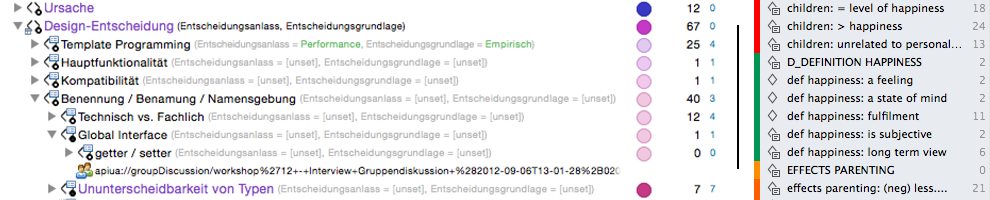
\includegraphics[width=1.0\linewidth]{Figures/apiua/codes-atlas.png}
  \caption[Vergleich APIUA und ATLAS.ti: Kode-Darstellung]{Vergleich Kode-Darstellung; links: \gls{apiua}; rechts: \textit{ATLAS.ti}}
  \label{fig:apiua-codes-atlas}
\end{figure}

\begin{figure}
  \centering
    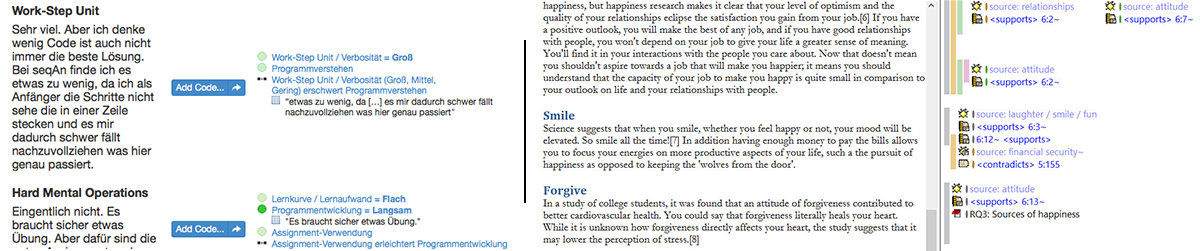
\includegraphics[width=1.0\linewidth]{Figures/apiua/codeinstances-atlas.png}
  \caption[Vergleich APIUA und ATLAS.ti: Kodeinstanz-Darstellung]{Vergleich Kodeinstanz-Darstellung; links: \gls{apiua}; rechts: \textit{ATLAS.ti}}
  \label{fig:apiua-codeinstances-atlas}
\end{figure}

\paragraph{Organisation und Sortierung von Kodes}
Im Gegensatz zur \textit{ATLAS.ti} können in \gls{apiua} Kodes gefiltert, sortiert und hierarchisch angeordnet werden (siehe \autoref{fig:apiua-codes-atlas}, links). Die Semantik der hierarchischen Modellierung wird von dem Werkzeug wie folgt behandelt: ``Wenn Kode \code{apiua://code/-9223372036854774936}\footnote{Zur Erinnerung: Es handelt sich hierbei um die Darstellung eines Kodes. Details zu dieser Stellung können im \sref{sec:notationen} auf Seite \pageref{sec:notationen} nachgelesen werden.} der Elter des Kodes \code{apiua://code/-9223372036854774934} ist, ist \code{apiua://code/-9223372036854774934} eine Ausprägung von \code{apiua://code/-9223372036854774936}, oder: \code{apiua://code/-9223372036854774936} manifestiert sich in \code{apiua://code/-9223372036854774934}.''

An dieser Stelle ist \textit{ATLAS.ti} scheinbar differenzierter. Dort können Beziehungen zwischen Elter und Kind von einer der drei Arten [\textit{Kategorie/generelles Konzept -- Kode}], [\textit{Oberbegriff -- Unterbegriff}] und [\textit{Das Ganze -- Bestandteile}] sein \citep{MuhlmeyerMentzel:2011vs}. Aber: Die Semantik dieser Beziehungen existiert nur in der Vorstellung des Forschers. Technisch handelt es sich lediglich um vordefinierte, benannte Relationstypen, die beliebig editiert werden können und von \textit{ATLAS.ti} selbst nicht weiter interpretiert werden. Im Gegensatz zu \gls{apiua} wird der Relationstyp in \textit{ATLAS.ti} nicht verwendet, um eine weitergehende Werkzeugunterstützung zu ermöglichen.

\cite{MuhlmeyerMentzel:2011vs} räumt ein, dass die Strukturierungsmöglichkeiten in \textit{ATLAS.ti} beschränkt sind. Insbesondere können Kodes nicht sortiert werden. Die Möglichkeit der hierarchischen Organisation von Kodes verändere den Arbeitsstil. Entschließt sich ein Forscher jedoch dazu, Kodes hierarchisch anzuordnen, kann er dies in \textit{ATLAS.ti} nur über die Definition von individuellen Relationen simulieren, die von der Anwendung aber nicht weiter berücksichtigt und beispielsweise nicht zur Darstellung eines Kode-Baums verwendet wird.

In \gls{apiua} kann jedes Datum, das \textit{Locatable} implementiert, auch kodiert werden. Da Kodes auch \textit{Locatable} implementieren, können Kodes andere Kodes kodieren. Um die Modellierungskomplexität nicht unnötig zu erhöhen, habe ich mich dazu entschlossen, diese Semantik mit der Eltern-Kind-Beziehung gleichzusetzen. Ist also \code{apiua://code/-9223372036854774934} ein Kind von \code{apiua://code/-9223372036854774936}, wird dies von \gls{apiua} genauso gehandhabt, als wäre \code{apiua://code/-9223372036854774934} mit \code{apiua://code/-9223372036854774936} kodiert worden.

Die eben beschriebene Beziehung gilt auch transitiv. Hat \code{apiua://code/-9223372036854774934} neben seinem Elternkode \code{apiua://code/-9223372036854774936} auch noch den Unterkode \code{apiua://code/-9223372036854774932}, so gilt: ``\code{apiua://code/-9223372036854774932} ist mit \code{apiua://code/-9223372036854774934} kodiert'' und ``\code{apiua://code/-9223372036854774932} ist mit \code{apiua://code/-9223372036854774936} kodiert''.

\paragraph{Memos} werden in APIUA umfassend unterstützt. Jedes Datum, das das \texttt{Locatable}-Interface implementiert, kann ein Memo besitzen. Das Memo des aktuell fokussierten Elements, erscheint im Memo-Editor (siehe \fref{fig:apiua-memos}). Ist das Fokus habende Element ein Kode oder eine Relation, werden optional auch sämtliche Memos der entsprechenden Kode- bzw. Relationsinstanzen gezeigt. Der Memo-Editor ist ein erweiterter, auf dem \textit{Nebula}-Browser basierender Rich-Text-Editor, der sowohl interne als auch externe Verknüpfungen zu anderen Daten erlaubt. Eine interne Verknüpfung bezieht sich auf eine \gls{uri} mit dem Schema \textit{apiua}. Klickt der Anwender auf einen solchen Link, öffnet dieser den Datenpunkt entsprechend seines Typs: Memo wird im Memo-Editor geladen, Kode wird in Kode-Ansicht hervorgehoben, Quellcode-Datei wird in der Vergleichsansicht geöffnet, etc. Verweilt der Anwender mit seiner Maus hingegen für einen kurzen Moment über einem Link (ohne ihn anzuklicken), so öffnet sich ein gelbes Informationsfenster, das wichtige --- wiederum typabhängige --- Informationen zu diesem Datenpunkt anzeigt (siehe \fref{fig:apiua-browsing}). Dieses Informationsfenster kann von anderen Plugins erweitert werden.

\begin{figure}
  \centering
    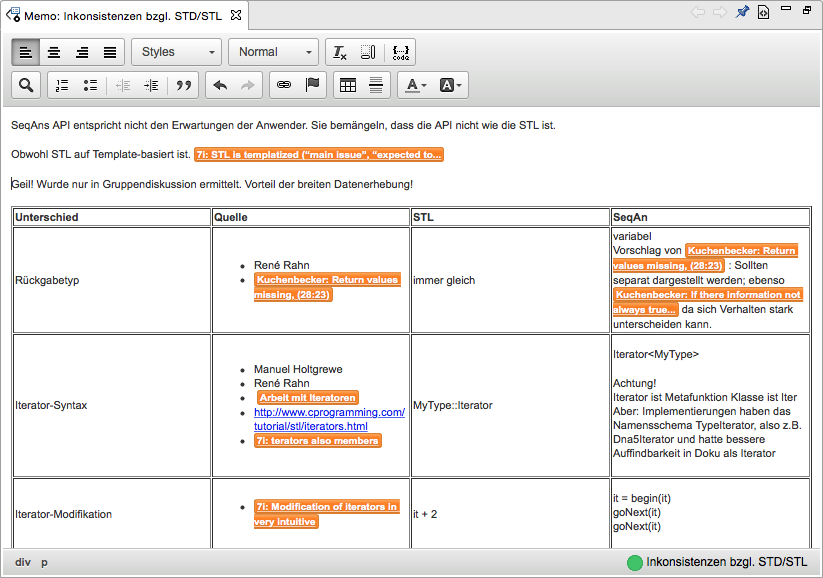
\includegraphics[width=0.8\linewidth]{Figures/apiua/memos.png}
  \caption[APIUA: Memo-Editor]{Dieser Screenshot zeigt den auf dem \textit{Nebula}-Browser basierenden Memo-Editor samt Inhalt für den Kode \url{apiua://code/-9223372036854775633}.}
  \label{fig:apiua-memos}
\end{figure}

\paragraph{Visualisierung}
Wie in \textit{ATLAS.ti} auch, können Kodes mit Farben versehen werden. Allerdings wird die Bedienung dieser Funktion von \cite{Zieris:yCXyxVc9} als umständlich und nicht für große Datenmengen geeignet, beschrieben. In \gls{apiua} kann der Anwender die Farbe eines spezifischen Kodes, eines Teilbaums oder des gesamten Kode-Bestands automatisch färben lassen. Die zweite und dritte Option skalieren auch für große Datenmengen gut. Dazu werden die Farben der Nachbarknoten berücksichtigt und ein konfliktfreier Farbraum bestimmt. Dieser wird dann rekursiv auf die Kindkodes gleich verteilt. Dadurch erhalten Kodes, die sich nah sind (gleicher Teilbaum, wenig Abstand zum Nachbarkode) eine ähnlichere Farbe als solche, die weiter voneinander entfernt sind. \fref{fig:apiua-colors} zeigt ein Beispiel. Diese Funktion hat sich als sehr nützlich für das axiale Kodieren erwiesen, da ich so ein besseren Überblick über verwandte Konzepte hatte.

\begin{figure}
  \centering
    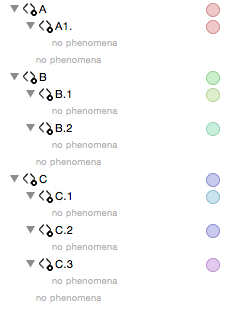
\includegraphics[width=0.4\linewidth]{Figures/apiua/colors.png}
  \caption[APIUA: Gruppendiskussion]{Dieser Screenshot von \gls{apiua} zeigt einen Kode-Teilbaum, der automatisch eingefärbt wurde. Auf den Elternkodes \code{apiua://code/-9223372036854774928}, \code{apiua://code/-9223372036854774927} und \code{apiua://code/-9223372036854774926} wird das gesamte Farbspektrum von Rot über Grün bis hin zu Violett verwendet. Die Kindkodes erhalten Farben, die links und rechts von der Elternfarbe liegen ohne den Bereich eines Nachbarteilbaums zu verletzen. Beispiel: Die Farbe von \code{apiua://code/-9223372036854774924} liegt links von \code{apiua://code/-9223372036854774927}; die von \code{apiua://code/-9223372036854774923} rechts davon.}
  \label{fig:apiua-colors}
\end{figure}

\paragraph{Eigenschaften}
In \gls{apiua} kann jeder Kode eine Dimension haben. Die zugrunde liegende Skala kann aktuell nominal oder ordinal sein\footnote{Die zur Verfügung stehenden Skalentypen können durch Plugins erweitert werden.}. Dimensionalisierte Kodes können als Eigenschaften anderer Kodes dienen. Ist ein Phänomen mit einem Kode kodiert worden, können dem Phänomen, in Bezug auf die Dimension und Eigenschaften des Kodes, Werte zugewiesen werden (siehe \autoref{fig:apiua-properties}).
\\Beispiel: Der Kode \code{Auto} verfügt über eine Eigenschaft \code{Farbe} mit der nominalen Skala \textit{(Rot, Gelb, Grün, Blau)}. Wird nun ein Phänomen \code{X} mit \code{Auto} kodiert, kann \code{X} nun ein Wert für die \textit{Farbe} zugewiesen werden, denn \code{X} ist fortan eine Instanz/Ausprägung/Phänomen für \code{Auto}.

Diese Art der Implementierung der \gls{gtm} erlaubt sogar \textit{Subdimensionalisierung} \citep{strauss1987qualitative}, also die Modellierung von Eigenschaften, die selbst wiederum Eigenschaften besitzen. Am Beispiel der Autofarbe könnte eine Untereigenschaft von Farbe die Eigenschaft \textit{Lackierung} \textit{(matt, glänzend)} sein.

\paragraph{Schwierigkeiten der Modellierung} von Analyseergebnissen ergeben sich bei der Verwendung hierarchischer Kodes und Eigenschaften:

\begin{description}
  \item[Spezifität] \hfill \\
  Während der Analyse meiner subjektiven Daten musste ich feststellen, dass die getroffenen Aussagen inhaltlich derart in die Breite gingen, dass ich für jeden generierten Kode kaum eine nennenswerte Zahl Verankerungen hatte. In solch einem Fall könnte man \textit{theoretischen Samplings} betreiben, indem man weitere Daten erhebt, um diese Kodes besser verstehen zu können. Allerdings kann eine solche Datenerhebung sehr teuer sein und ein Mittelweg muss gefunden werden.
  
  Konkretes Beispiel: In meinen Daten schildert\citepurl{apiua://survey/cd/2013-09-19T11:51:16.616+02:00/hardMentalOperations} ein Proband seine Frustration von dem Templatemetaprogrammiungs-Aspekt \textit{Metafunktion}, was ich mit dem Kode \code{apiua://code/-9223372036854775514} kodierte. Dieser Kode ist selbst ein Unterkode von \code{apiua://code/-9223372036854775515}. An anderer Stelle gibt es eine weniger spezifische Aussage\citepurl{apiua://survey/cd/2013-09-19T11:51:16.616+02:00/workStepUnit}, in der nur noch allgemein von \textit{Templatemetaprogramming} die Rede ist.
  
  \medskip
  
  \begin{center}
    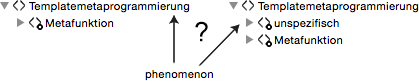
\includegraphics[width=0.7\linewidth]{Figures/apiua/problem-specificity.png}
  \end{center}
  
  Hier stellt sich nun die Frage, ob die allgemeinere Aussage mit \code{apiua://code/-9223372036854775515} kodiert werden sollte. Oder man führt einen ``unspezifischen'' Unterkode von \code{apiua://code/-9223372036854775515} ein und verwendet diesen dann als ``Sammelbecken'' für Phänomene mit geringerem Aussagegehalt.
  
  
  
  \item[Vererbung] \hfill \\
  Welche Auswirkungen haben Eigenschaften eines Kodes auf seine Eltern- bzw. Kindkodes? Denkt man an Objektorientierung, hieße die Antwort, dass Eigenschaften nach unten vererbt werden. Aber gilt das auch für Kodeinstanzen? Würden wir uns beim obigen Beispiel für die erste Variante entscheiden, würde das Phänomen nicht nur eine Instanz von \code{apiua://code/-9223372036854775515} darstellen, sondern auch von allen Unterkodes von \code{apiua://code/-9223372036854775515}, u.a. auch \code{apiua://code/-9223372036854775514}. Ob sich ein Phänomen auf alle Unterformen bezieht oder schlichtweg nur eine geringe Aussagekraft hat, kann man nicht immer zuverlässig sagen. Oder gilt die Vererbung von Kodeinstanzen gar nach oben? Immerhin sollten sich Aussagen über \code{apiua://code/-9223372036854775515} treffen lassen, wenn man konkretere Phänomene zu \code{apiua://code/-9223372036854775514} gesehen hat. 
  
  Meinen Lösungsvorschlag für diese Problemfragen gebe ich weiter unten. 
\end{description}

\begin{figure}
  \centering
    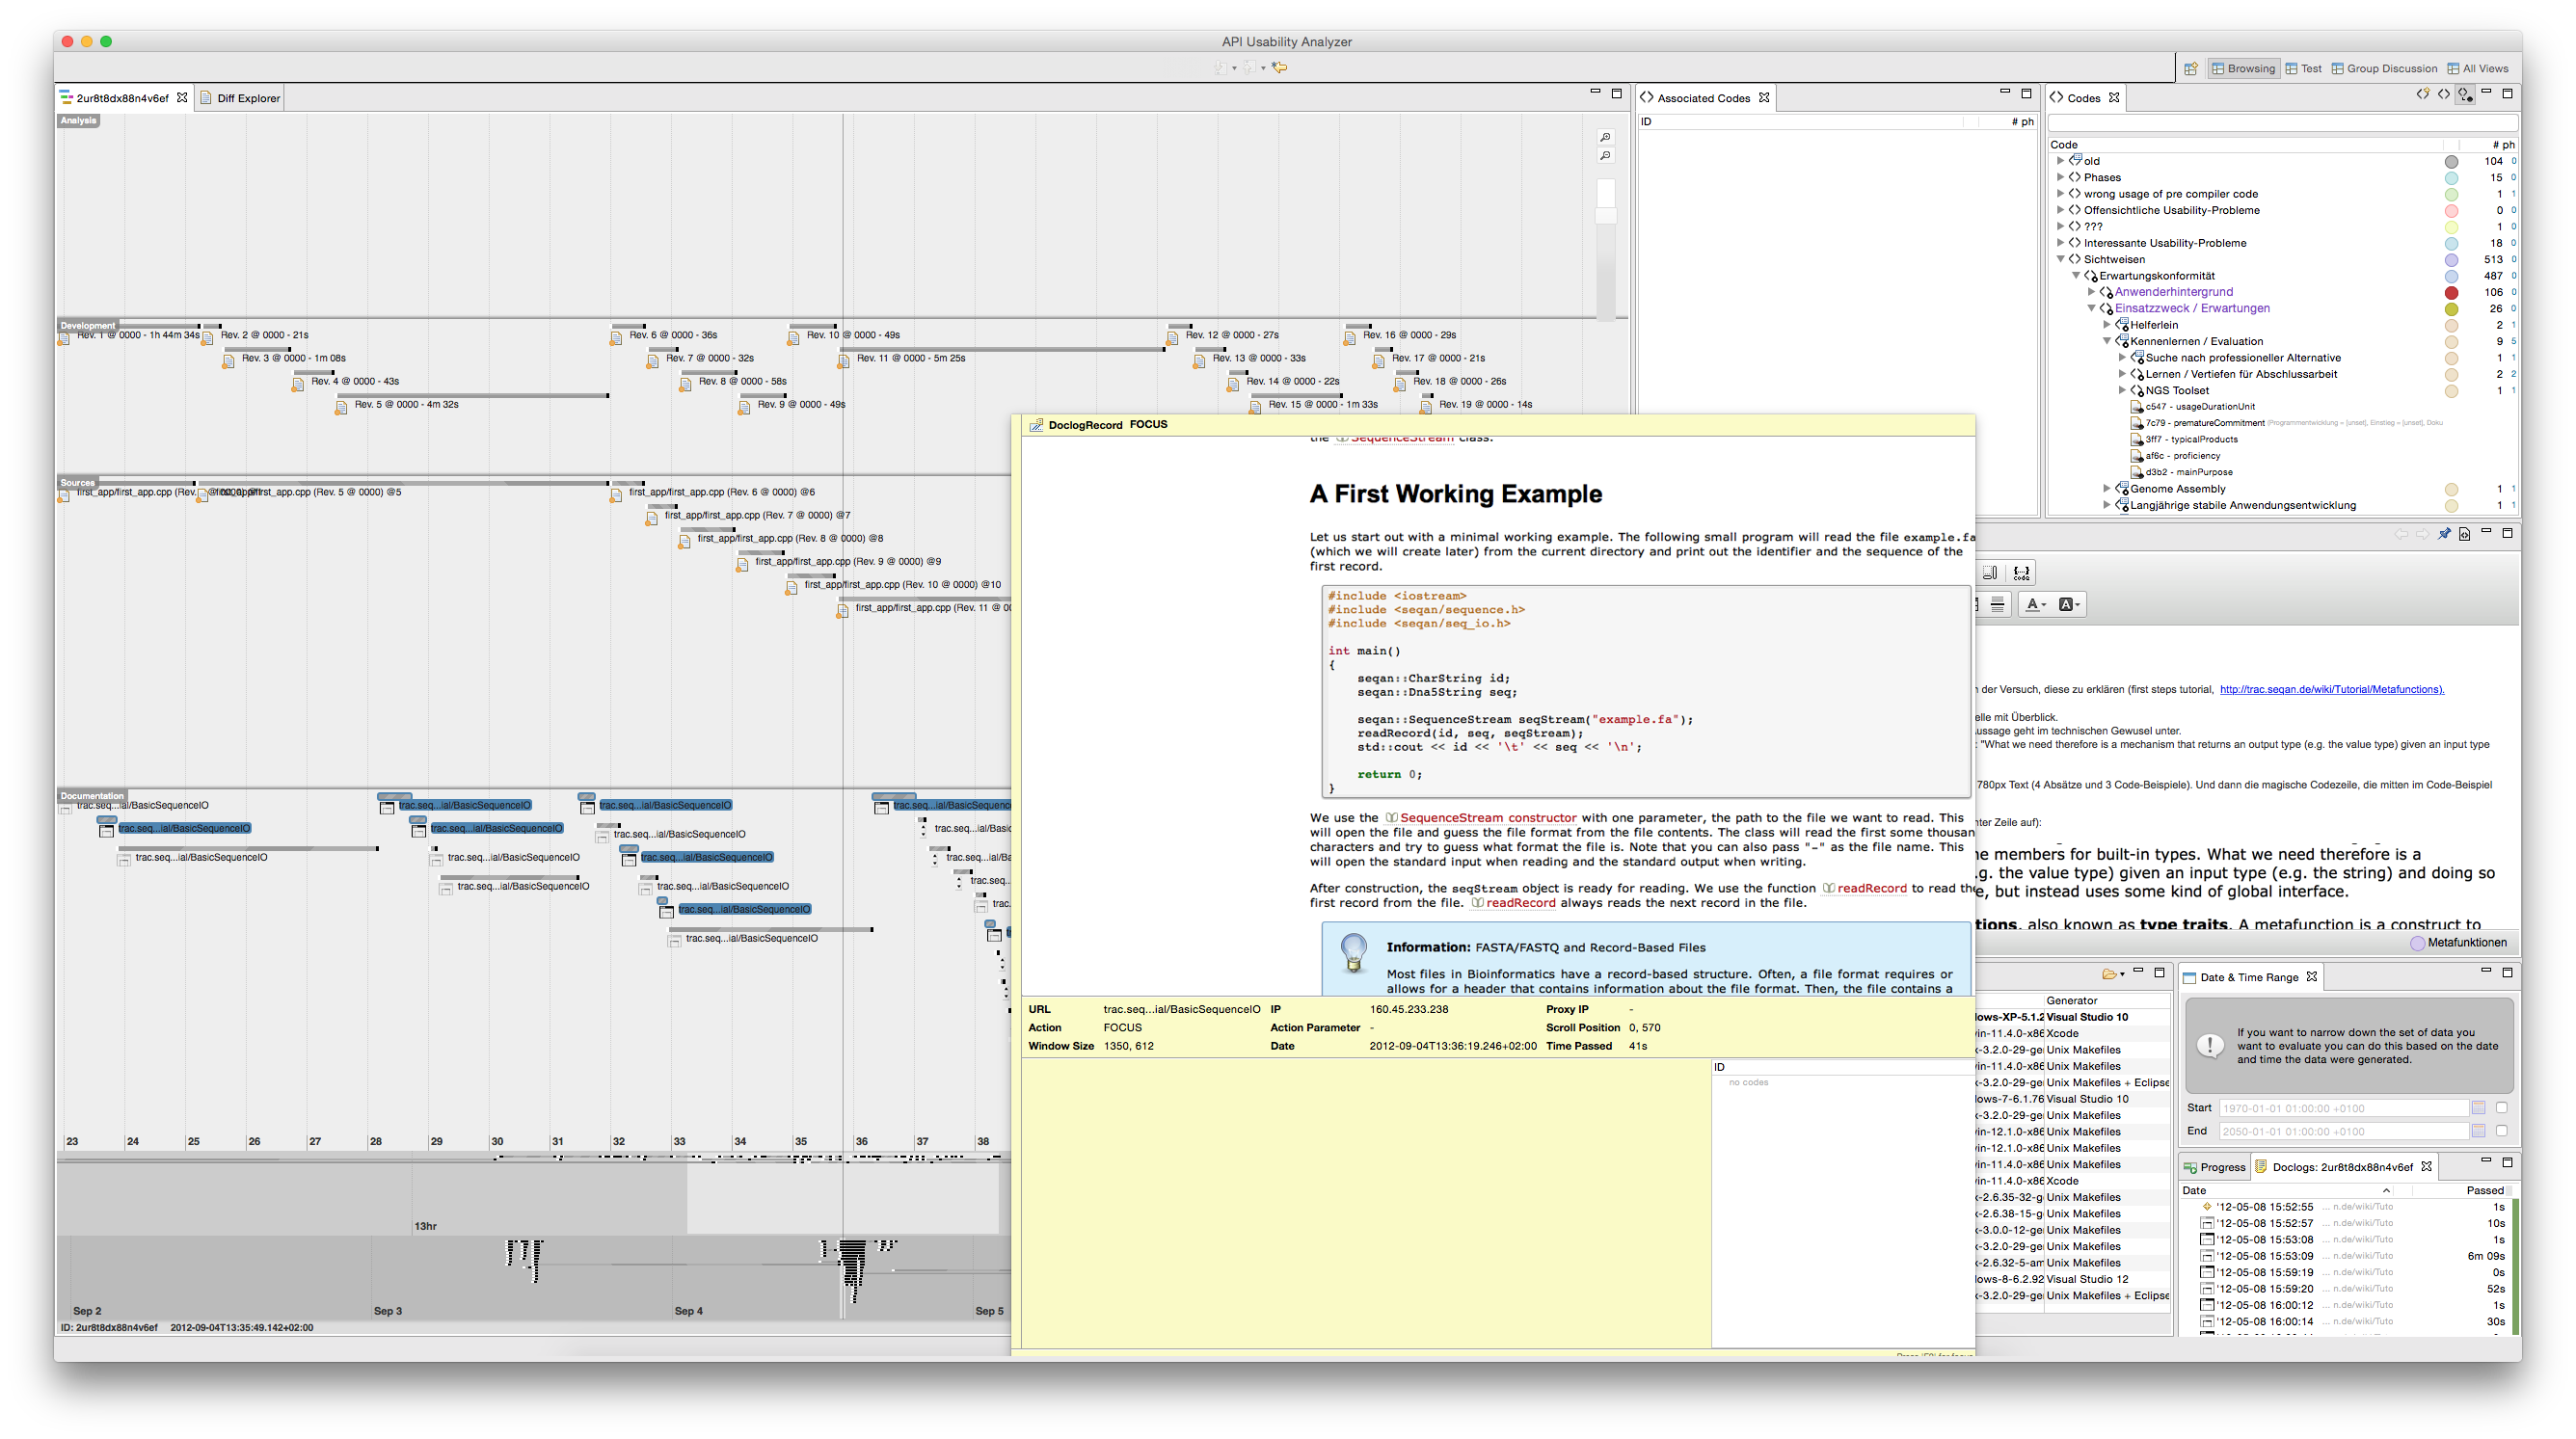
\includegraphics[width=1.0\linewidth]{Figures/apiua/browsing.png}
  \caption[APIUA: Exploration]{Dieser Screenshot von \gls{apiua} zeigt eine typische Analysesitzung, bei der sich der Forscher einen Überblick über die Daten verschafft. Dazu nutzt er die Zeitleistenansicht.}
  \label{fig:apiua-browsing}
\end{figure}

\begin{figure}
  \centering
    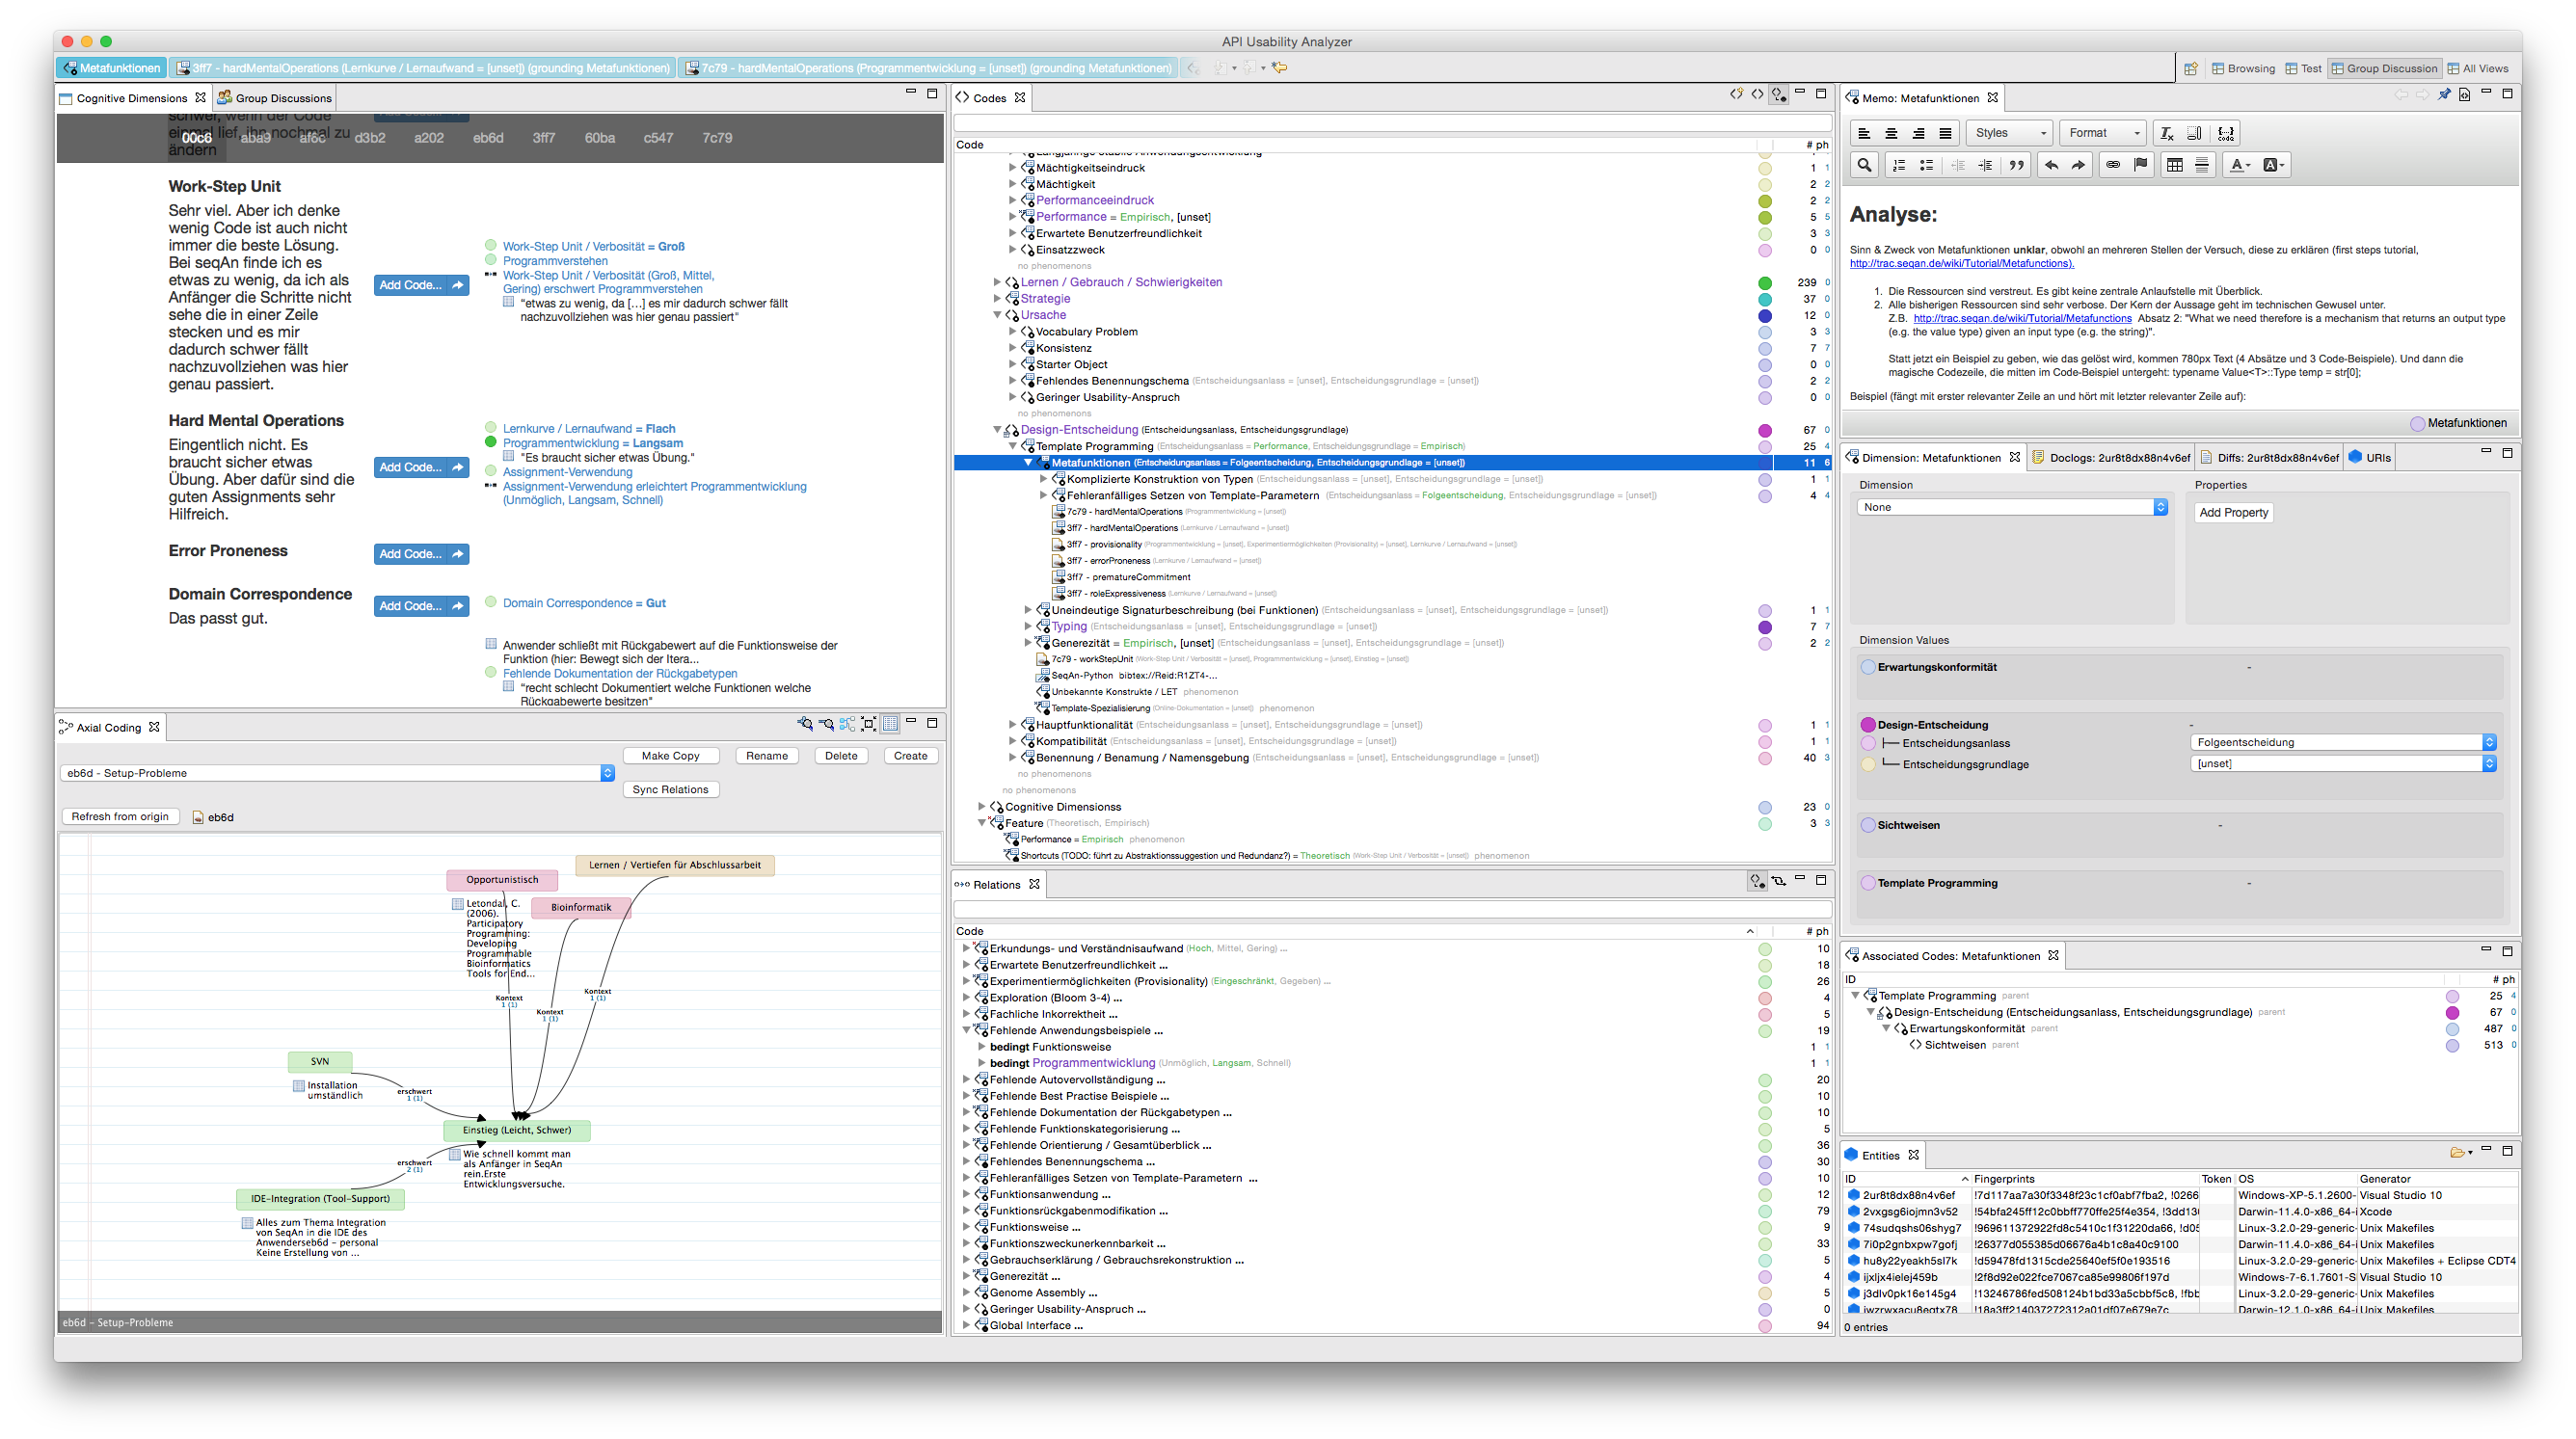
\includegraphics[width=1.0\linewidth]{Figures/apiua/opencoding-cd.png}
  \caption[APIUA: Cognitive Dimensions]{Dieser Screenshot von \gls{apiua} zeigt eine typische Sitzung mit Fokus auf offenes Kodieren. In diesem Fall werden die Cognitive-Dimensions-Fragebögen (oben links) analysiert.}
  \label{fig:apiua-opencoding-cd}
\end{figure}

\begin{figure}
  \centering
    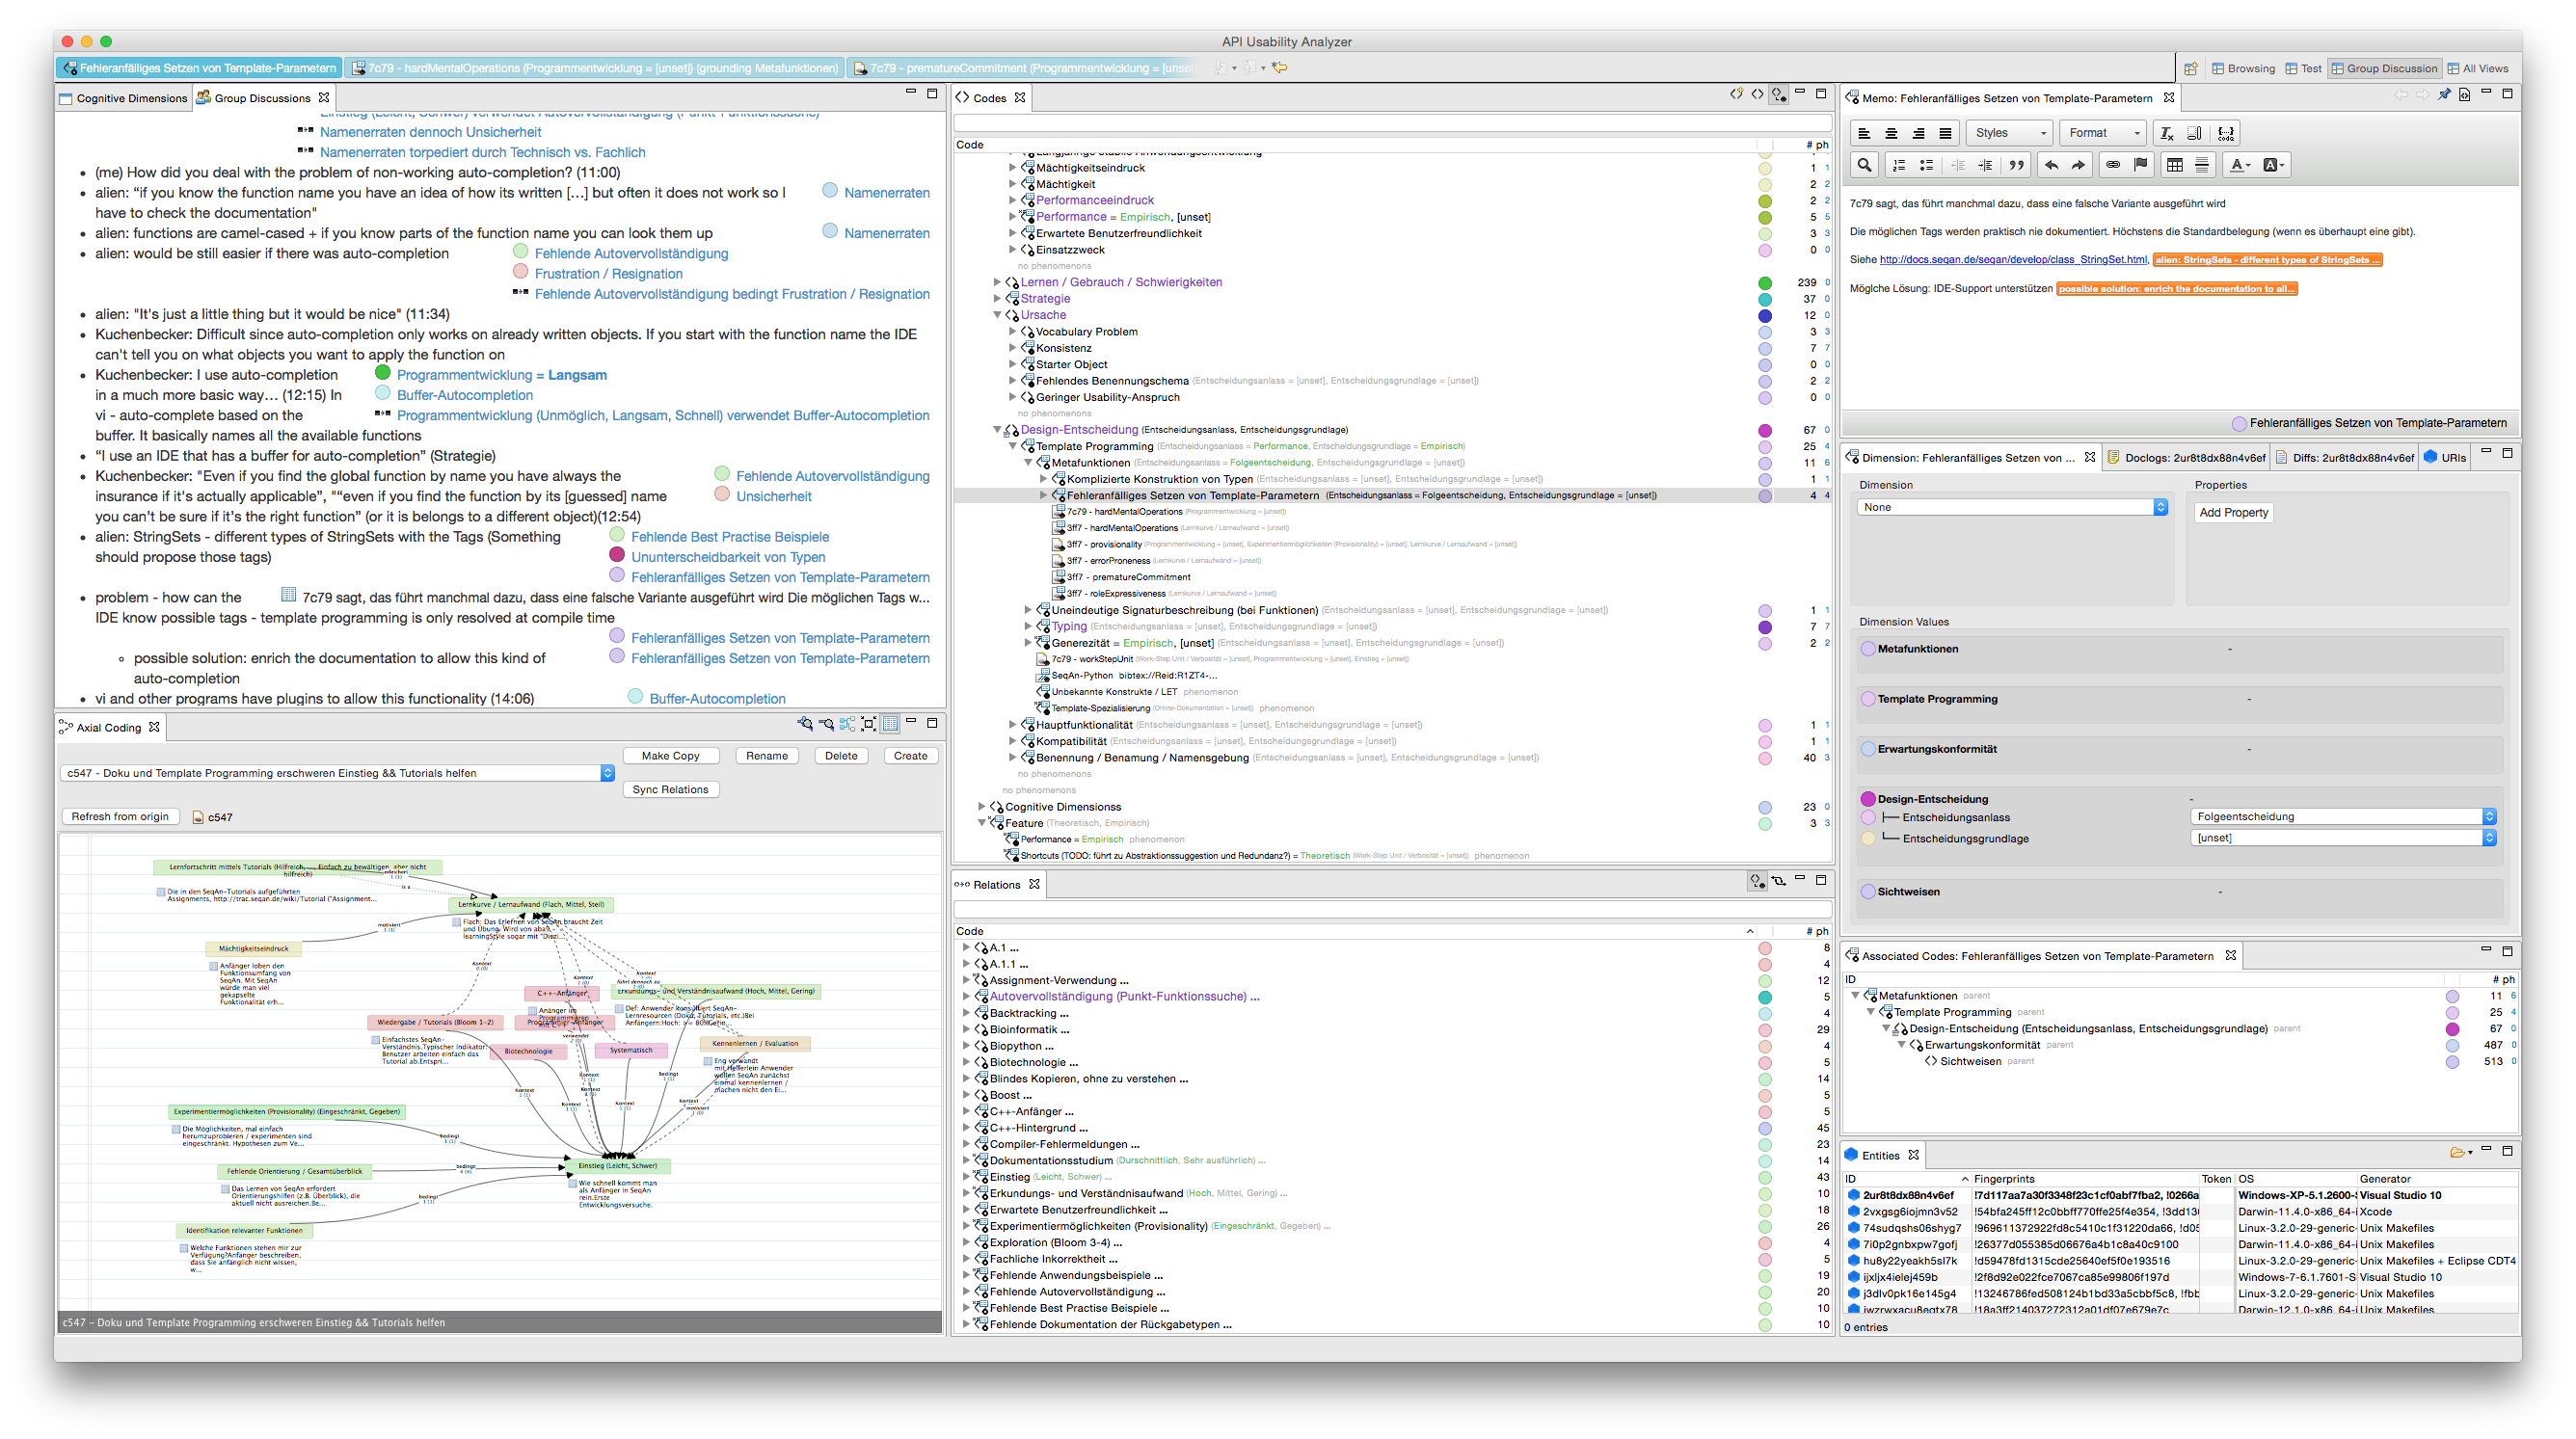
\includegraphics[width=1.0\linewidth]{Figures/apiua/opencoding-gd.png}
  \caption[APIUA: Gruppendiskussion]{Dieser Screenshot von \gls{apiua} zeigt eine typische Sitzung mit Fokus auf offenes Kodieren. In diesem Fall wird eine Gruppendiskussion (oben links) betrachtet.}
  \label{fig:apiua-opencoding-gd}
\end{figure}

Nach der \gls{gtm} von \cite{strauss1990basics,corbin2014basics} ``darf'' auch das Vorwissen des Forschers in den Forschungsprozess eingebracht werden. Die \textit{\acrshort{uri}}-Komponente von \acrshort{apiua} erlaubt das Erfassen \acrshort{uri}-referenzierbarer Quellen. Dies ermöglicht es dem Forscher Konzepte in beliebigen Dokumenten zu verankern, auf das sein Vorwissen fußt. In meiner Forschung habe ich Verankerungen ganz konkret auf Basis von Literatur mit Hilfe von \url{bibtex:}-\acrshort{uri}s und verschiedenartigste Dokumente mit Hilfe von \url{file:}-\acrshort{uri}s vorgenommen. Dieses Vorgehen ist aus meiner Sicht unerlässlich, um die Gütekriterien \textit{Argumentative Interpretationsabsicherung} und \textit{Nähe zum Gegenstand} zu erfüllen. Keines der mir bekannten CAQDAS-Anwendungen erfüllt diese Anforderungen, ohne dass die referenzierten Dokumente auch direkt in das Datenanalysewerkzeug importiert und damit auch von dem Werkzeug unterstützt werden müssten.




\subsubsection{Axiales Kodieren}
\label{sec:apiua-axial-coding}

Die Möglichkeit axial kodieren zu können, ist ein integraler Bestandteil von \gls{apiua}. Eine Relation in \gls{apiua} ist wie ein benannter gerichteter Graph zwischen zwei Kodes und wird in dieser Arbeit wie folgt notiert: \rel[Bezeichner]{\code{Kode 1}}{\code{Kode 2}}. \autoref{fig:apiua-axialcoding} zeigt die entsprechende Ansicht in APIUA. So wie Kodes mit Hilfe von Kodeinstanzen verankert werden, können auch Relationen mittels Relationsinstanzen verankert werden.

\textit{ATLAS.ti} verwendet zwar für Kodes ein vergleichbares Datenmodell \citep{MuhlmeyerMentzel:2011vs}, kann aber Relationen selbst nicht verankern \citep{Zieris:yCXyxVc9}. Möchte der Forscher also nachschauen, auf welchen Datenpunkten eine Relation überhaupt fußt, besteht für ihn nur die Möglichkeit, alle Stellen zu ermitteln, die als Verankerungen für die beiden, durch die Relation in Beziehung gesetzten Kodes dienen und in Gedanken neu zu kodieren.

Kurzum: Wenn der Forscher das Verankerungsproblem nicht auf andere Weise gelöst hat, können Verankerungen von Relationen durch Dritte nur eingeschränkt nachvollzogen werden, was aus meiner Sicht die Verifizierbarkeit von mit \textit{ATLAS.ti} erstellten Relationen potentiell einschränkt.

Eine weitere Einschränkung in \textit{ATLAS.ti} besteht darin, dass es zwischen zwei Kodes nur eine Relation geben kann. \gls{apiua} unterstützt beliebig viele --- wenn der Forscher es für notwendig hält auch gleich benannte --- Relationen.

\begin{figure}
  \centering
    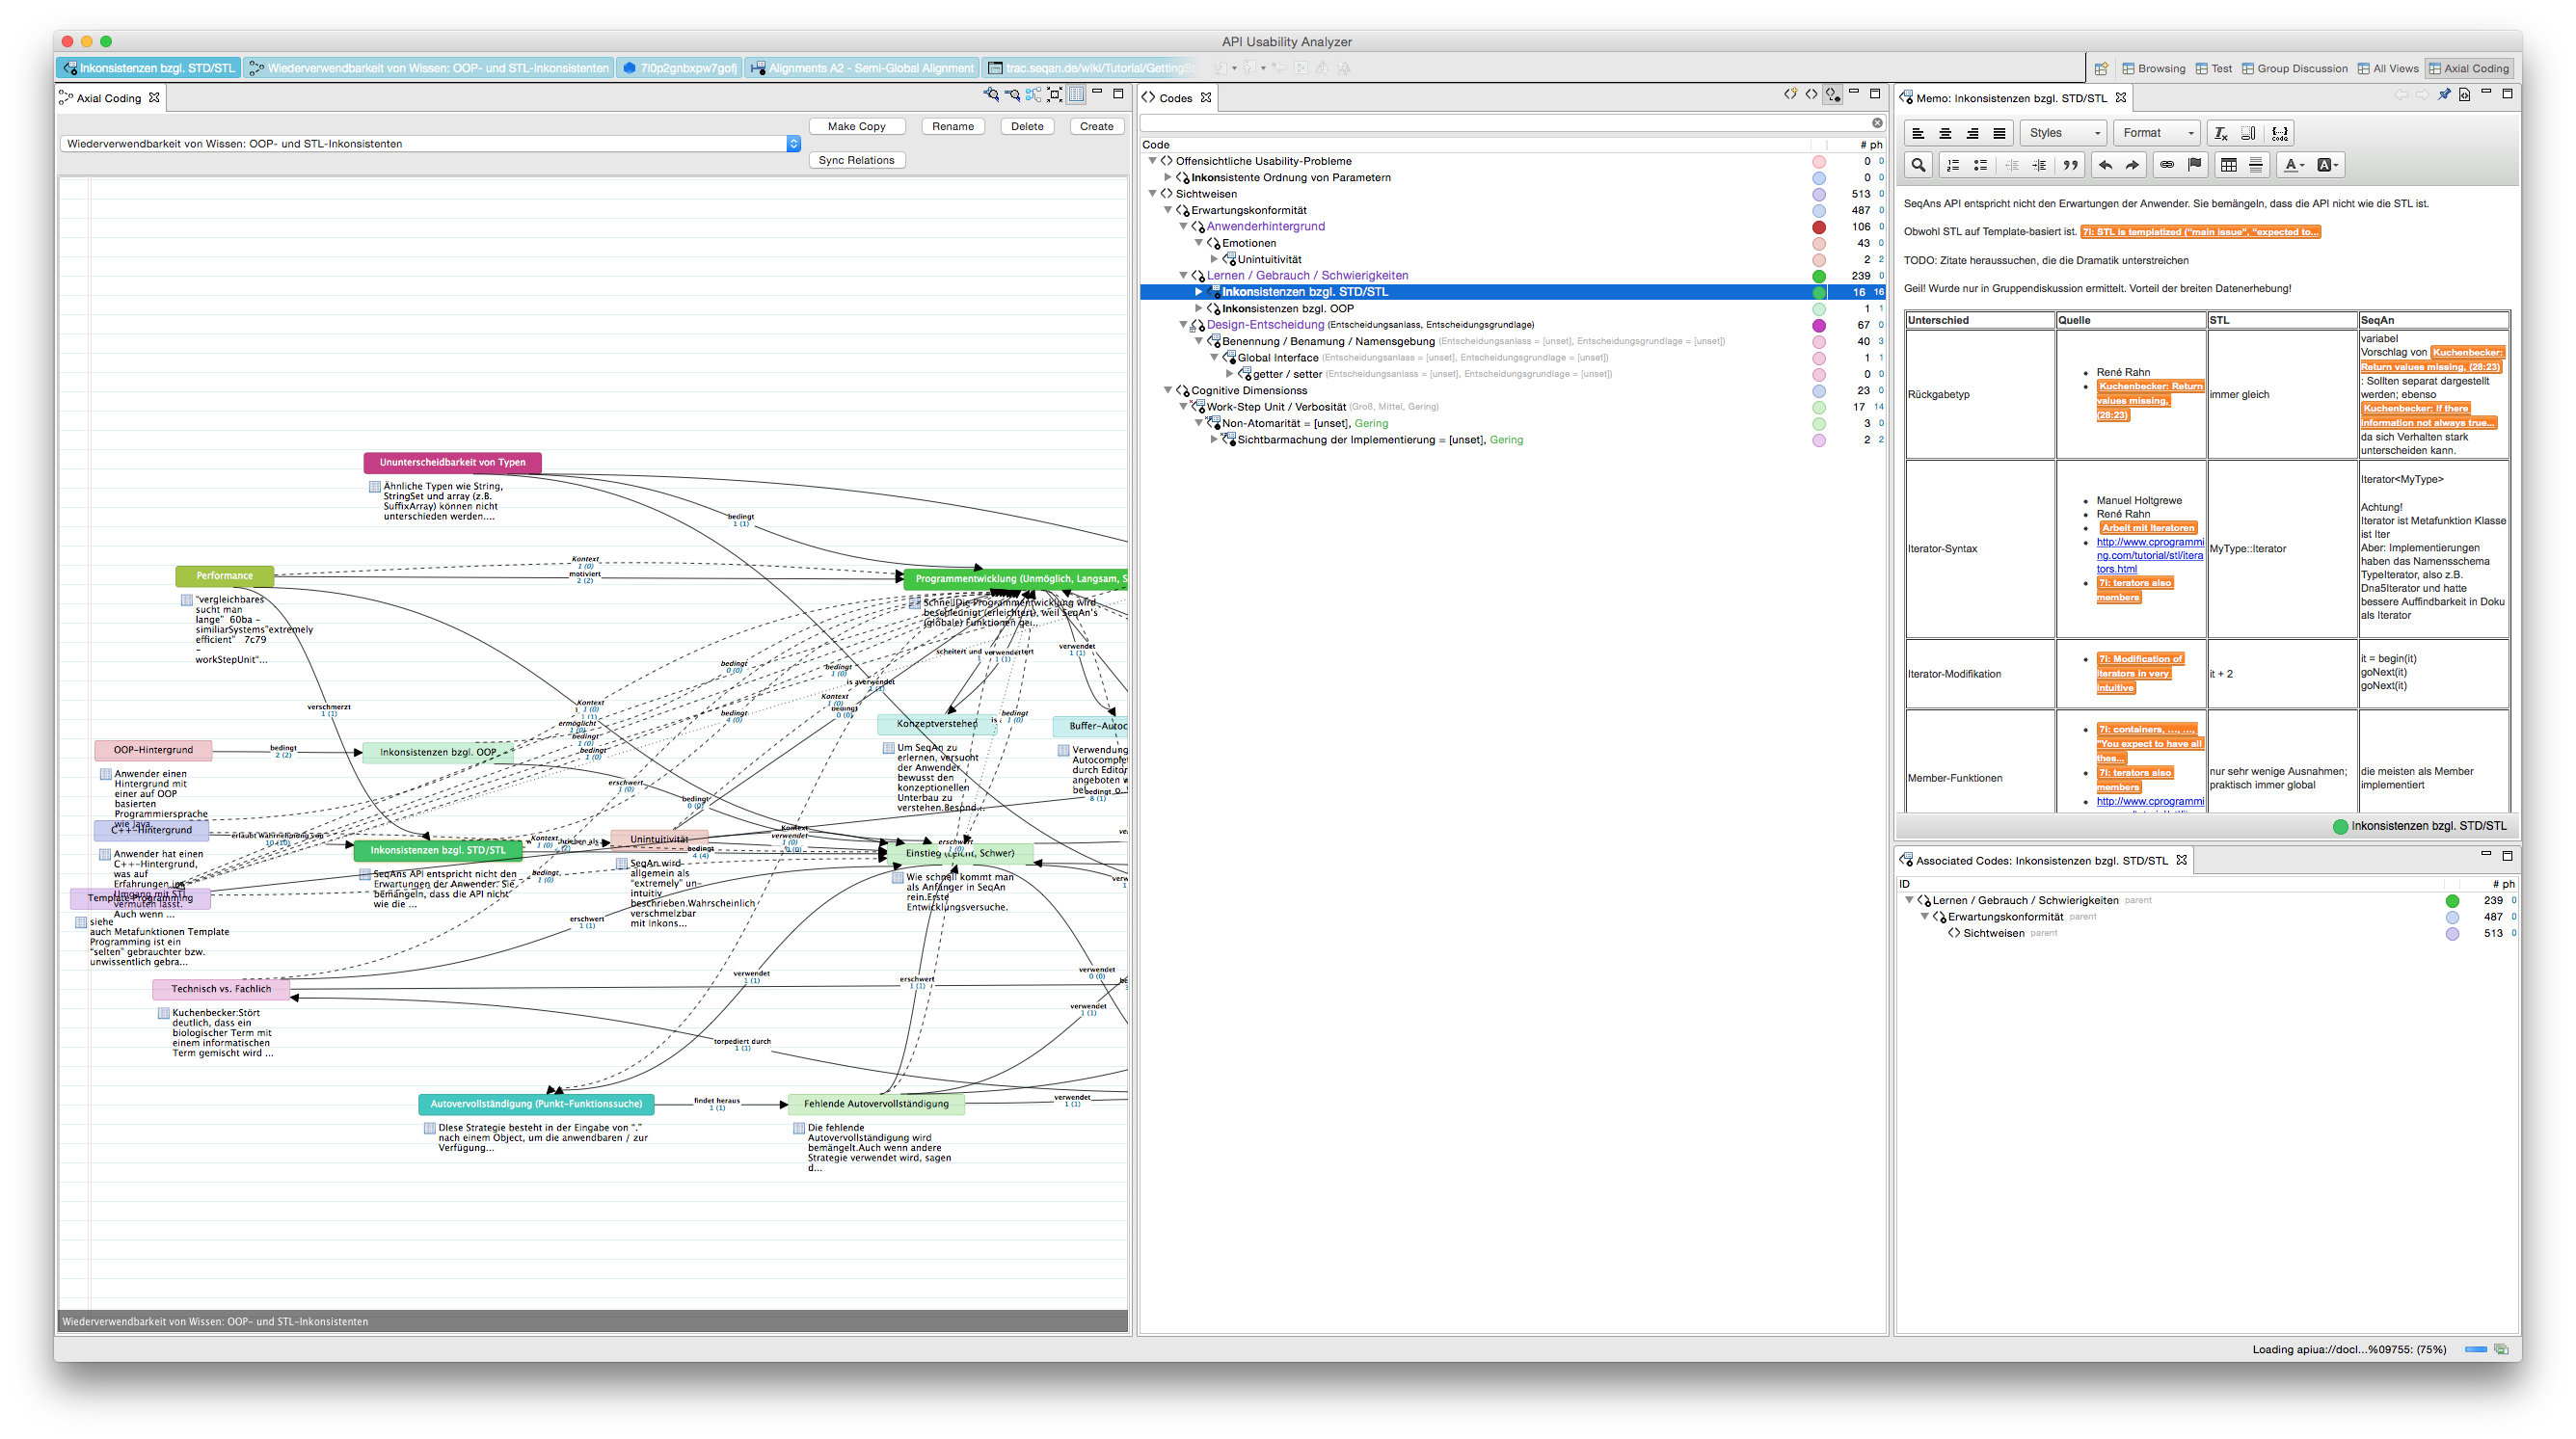
\includegraphics[width=1.0\linewidth]{Figures/apiua/axialcoding.png}
  \caption[APIUA: Axiales Kodieren ]{Dieser Screenshot von \gls{apiua} zeigt eine typische Sitzung mit Fokus auf axiales Kodieren. In diesem Fall wird das \glslink{acm}{axiale Kodiermodell} ``OOP- u. STL-Inkonsistenzen'' --- links dargestellt --- bearbeitet.}
  \label{fig:apiua-axialcoding}
\end{figure}

Der Forscher hat zwei verschiedene Möglichkeiten \glspl{ac} bzw. \glspl{acm}\footnote{Zur Erinnerung: Eine \gls{ac} stellt Relationen auf Kodeinstanz-Ebene dar, wohingegen ein \gls{acm} Relationen auf Kode-Ebene beschreibt.} zu erstellen. Entweder beginnt er ``from scratch'', entwickelt also eines von Grund auf oder er erstellt eines auf der Grundlage eines existierenden Kodes, einer existierenden Relation oder einer jeweiligen Instanz. In beiden Fällen hält der Editor den Graphen bei Änderungen (Umbenennungen, Farbänderungen, Hierarchieänderungen, etc.) aktuell. Im zweiten Fall wird darüber hinaus der Graph selbst dynamisch erzeugt, initial formatiert und ebenfalls aktuell gehalten. Der so erstellte Graph enthält alle Kodes bzw. Kodeinstanzen, mit denen der ursprünglich ausgewählte Kode bzw. die Kodeinstanz über Relationen verbunden ist. Gibt es also \rel{\code{apiua://code/-9223372036854774936}}{\code{apiua://code/-9223372036854774935}} und basiert der Graph auf \code{apiua://code/-9223372036854774936}, enthält der Graph neben \code{apiua://code/-9223372036854774936} auch \code{apiua://code/-9223372036854774935} und \rel{\code{apiua://code/-9223372036854774936}}{\code{apiua://code/-9223372036854774935}}. Für Elemente, die für den Aussagekern des \glslink{acm}{axialen Kodiermodells} unwichtig sind, besteht die Möglichkeit, sie auszublenden.

Zurück zum obigen Beispiel: Ein Proband machte eine Aussage\citepurl{apiua://survey/cd/2013-09-19T11:51:16.616+02:00/hardMentalOperations} zu Metafunktionen. Genauer: Die Notwendigkeit, sich mit Metafunktionen auseinanderzusetzen, wird als frustrierend beschrieben. Daraus ergibt sich \rel[bedingt]{\code{apiua://code/-9223372036854775514}}{\code[apiua://code/-9223372036854775314]{Frustration/Resignation}}. Eine andere Aussage\citepurl{apiua://survey/cd/2013-09-19T11:51:16.616+02:00/workStepUnit} ist ähnlich, aber weniger spezifisch: \rel[bedingt]{\code{apiua://code/-9223372036854775515}}{\code[apiua://code/-9223372036854775314]{Frustration/Resignation}}.

Durch die Unterstützung von Unter- und Überkodes könnte man nun definieren, dass \rel[bedingt]{\code{apiua://code/-9223372036854775514}}{\code[apiua://code/-9223372036854775314]{Frustration/Resignation}} eine Unterrelation von \rel[bedingt]{\code{apiua://code/-9223372036854775515}}{\code[apiua://code/-9223372036854775314]{Frustration/Resignation}} ist. Oder allgemeiner: Ist \code{apiua://code/-9223372036854774934} Unterkode von \code{apiua://code/-9223372036854774936} und \code{apiua://code/-9223372036854774933} Unterkode von \code{apiua://code/-9223372036854774935}, wären \rel[x]{\code{apiua://code/-9223372036854774934}}{\code{apiua://code/-9223372036854774935}}, \rel[x]{\code{apiua://code/-9223372036854774936}}{\code{apiua://code/-9223372036854774933}} und \rel[x]{\code{apiua://code/-9223372036854774934}}{\code{apiua://code/-9223372036854774933}} Unterrelationen von \rel[x]{\code{apiua://code/-9223372036854774936}}{\code{apiua://code/-9223372036854774935}} (\textit{x} ist ein beliebiger gemeinsamer Bezeichner; siehe \autoref{fig:SubRelations}).

\begin{figure}
  \centering
    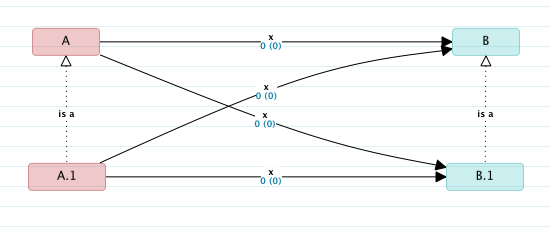
\includegraphics[width=1.0\linewidth]{Figures/sub_relations.png}
  \caption[APIUA: Modellierung --- Unterrelationen]{Die Relationen \rel[x]{\code{apiua://code/-9223372036854774934}}{\code{apiua://code/-9223372036854774935}}, \rel[x]{\code{apiua://code/-9223372036854774936}}{\code{apiua://code/-9223372036854774933}} und \rel[x]{\code{apiua://code/-9223372036854774934}}{\code{apiua://code/-9223372036854774933}} sind Unterrelationen von \rel[x]{\code{apiua://code/-9223372036854774936}}{\code{apiua://code/-9223372036854774935}}.}
  \label{fig:SubRelations}
\end{figure}

Auch diese Konstruktion ist wie bei den Kodes transitiv. Hätte \code{apiua://code/-9223372036854774934} den Unterkode \code{apiua://code/-9223372036854774932} und \code{apiua://code/-9223372036854774933} den Unterkode \code{apiua://code/-9223372036854774931} und gäbe es die Relationen \rel[x]{\code{apiua://code/-9223372036854774936}}{\code{apiua://code/-9223372036854774935}}, \rel[x]{\code{apiua://code/-9223372036854774934}}{\code{apiua://code/-9223372036854774933}} und \rel[x]{\code{apiua://code/-9223372036854774932}}{\code{apiua://code/-9223372036854774931}} so wäre nicht nur \rel[x]{\code{apiua://code/-9223372036854774934}}{\code{apiua://code/-9223372036854774933}} Unterrelation von \rel[x]{\code{apiua://code/-9223372036854774936}}{\code{apiua://code/-9223372036854774935}} sondern auch \rel[x]{\code{apiua://code/-9223372036854774934}}{\code{apiua://code/-9223372036854774933}} Unterrelation von \rel[x]{\code{apiua://code/-9223372036854774936}}{\code{apiua://code/-9223372036854774935}}.

So wie Kodes Kodeinstanzen haben können, können Relationen auch Relationsinstanzen besitzen. Hier stellt sich dieselbe Vererbungsfrage wie bei Kodes: Erben Unterrelationen die Instanzen ihrer Überrelation (oder anders herum)? Und wie kodiere ich unspezifische Aussagen?


\subsubsection{Selektives Kodieren}
\label{sec:apiua-selective-coding}

In \textit{ATLAS.ti} gibt es keine explizite Unterstützung für selektives Kodieren. Von dem Forscher wird erwartet, dass er dazu die vorhandene Funktionalität der Software nutzt. Dazu zählen insbesondere die für das axiale Kodieren bereitgestellten Möglichkeiten.

Ähnlich verfährt auch \gls{apiua} --- mit zwei Ausnahmen:
\begin{enumerate}
	\item \gls{apiua} implementiert in Ansätzen, die Möglichkeit, Interferenzregeln auf die erarbeitete theoretische Modellierung anzuwenden, was das selektive Kodieren unterstützen kann. Dabei handelt es sich um eine Funktion, die keine der mir bekannten Konkurrenzprodukte unterstützt.
	\item Darüber hinaus gibt es die Möglichkeit, einem Kode eine Hervorhebungsgruppe zuzuordnen. Standardmäßig werden Kodes nicht hervorgehoben. Der Anwender hat die Möglichkeit die Hervorhebung abzusenken --- die schwarze Kodebeschriftung wird dann plattformweit \textcolor{gray}{grau} und die Kodefarbe blass dargestellt --- oder sie anzuheben --- dann wird die Kodebeschriftung \textbf{\textcolor{violet}{fett und violett}} und die Kodefarbe kräftiger dargestellt (siehe \fref{fig:apiua-opencoding-cd}). Auf diese Weise kann der Forscher in jeder Phase seiner Forschung Kandidaten für selektives Kodieren festhalten.
\end{enumerate}




\subsubsection{Erkenntnisperspektive}
\label{sec:Erkenntnisperspektive}

In den vorangegangenen Abschnitten habe ich Fragen aufgeworfen, die die konkrete Modellierung einer \acrfull{gt} innerhalb eines Datenanalysewerkzeugs betreffen. Sie betreffen einerseits den Umgang mit Aussagen geringerer Spezifität und andererseits die Vererbung von Erkenntnissen. Diese Fragen stellten sich mir bei dem Versuch, automatisch generierte \glspl{gtm} zu verallgemeinern und ihre wesentliche Aussage herauszuarbeiten (siehe \sref{sec:Datenanalyse-STL-Inkonsistenzen-vereinfachen}).

Als \textit{Erkenntnisperspektive} bezeichne ich, ob der Forscher entweder gerade eine synthetische (abduktiv oder induktiv -- also ``Erkenntnis erweiternd'') oder deduktive \citep{Rehfus:2003ti} Sichtweise einnimmt. Während der Entwicklung einer \gls{gt} nimmt der Forscher häufig die synthetische Erkenntnisperspektive ein, denn in ihr besteht ja gerade der Erkenntnisgewinn. Genauso häufig aber wechselt er in die deduktive Erkenntnisperspektive, um seine Hypothesen zu überprüfen \citep{kelle1994empirisch}. Dieser Wechsel zwischen Induktion und Deduktion findet während des gesamten Forschungszeitraums statt \citep[siehe \sref{sec:gtm} und][]{strauss1987qualitative}.

Mit einer deduktiven Erkenntnisperspektive sollte es sich wie bei der Objektorientierung verhalten: Die Vererbung findet von oben nach unten statt. Aussagen, die ich für Überkodes bzw. Überrelationen treffen kann, müssen --- wenn die \gls{gt} funktioniert --- auch für deren Unterkodes bzw. Unterrelationen gelten\footnote{Ganz so streng ist die Prämisse nicht, und soll auch so nicht verstanden werden. Die theoretische Konstruktion verfügt lediglich über eine ``Aura der Objektivität'' (``aura of objectivity'') und darf nicht für ein ``erzwungenes Rahmenwerk'' (``forced framework'') gehalten werden. \citep{charmaz2006constructing}\\ Eine \gls{gt}, die tatsächlich jede Beobachtung vollumfänglich erklären kann, würde Gefahr laufen, sehr deskriptiv zu werden und sich nicht mehr dazu eignen, verallgemeinerbare Aussagen zu treffen.}. 

Mit einer synthetischen Erkenntnisperspektive hingegen kann man eine hypothetische Vererbung nach oben in Erwägung ziehen. So könnten Aussagen, die für Unterkodes gelten möglicherweise auch für den Überkode gelten.

\gls{apiua} soll den bereits von \cite{Glaser:1967ts} als erforderlich beschrieben Wechsel zwischen induktivem und deduktivem Denken --- insbesondere beim axialen Kodieren \citep{strauss1990basics} --- Werkzeug-seitig unterstützen. Darum ist \gls{apiua} dem Forscher beim Einnehmen der synthetischen Erkenntnisperspektive bereits jetzt schon behilflich, indem es zum Beispiel zwischen expliziten und impliziten Relationen unterscheidet. Eine explizite Relation \relation{R} ist eine, die vom Forscher modelliert wurde. Eine implizite Relation hingegen basiert auf einer anderen explizit definierten Relation \relation{R\_}, die selbst Unterrelation von \relation{R} ist und damit \relation{R} impliziert (siehe \autoref{fig:ImplicitRelations}). Existiert \relation{R} allerdings (noch) nicht, fungiert \relation{R\_} als hypothetische Relation für ein mögliches \relation{R}. %Oder genauer: \relation{R\_} stellt für alle erdenklichen Überrelationen eine hypothetische Relation dar (siehe Abbildungen \ref{fig:ProposedRelations1}, \ref{fig:ProposedRelations2} und \ref{fig:ProposedRelations3}).

\begin{figure}
  \centering
    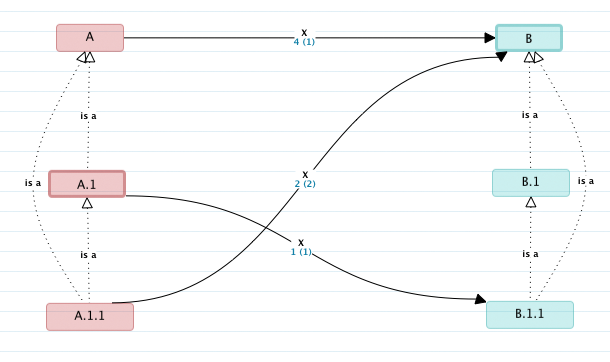
\includegraphics[width=1.0\linewidth]{Figures/implicit_relations.png}
  \caption[APIUA: Modellierung --- Implizite Relationen]{Die Relationen \rel[x]{\code{apiua://code/-9223372036854774934}}{\code{apiua://code/-9223372036854774931}}, sowie \rel[x]{\code{apiua://code/-9223372036854774932}}{\code{apiua://code/-9223372036854774935}} sind implizit für \rel[x]{\code{apiua://code/-9223372036854774936}}{\code{apiua://code/-9223372036854774935}}. Demnach erhöht sich die Verankerung von \rel[x]{\code{apiua://code/-9223372036854774936}}{\code{apiua://code/-9223372036854774935}} um die Summe der Verankerungen der impliziten Relationen ($1+2=3$). \rel[x]{\code{apiua://code/-9223372036854774936}}{\code{apiua://code/-9223372036854774935}} konnte also einmal direkt und dreimal indirekt verankert werden.}
  \label{fig:ImplicitRelations}
\end{figure}

\begin{figure}
  \centering
    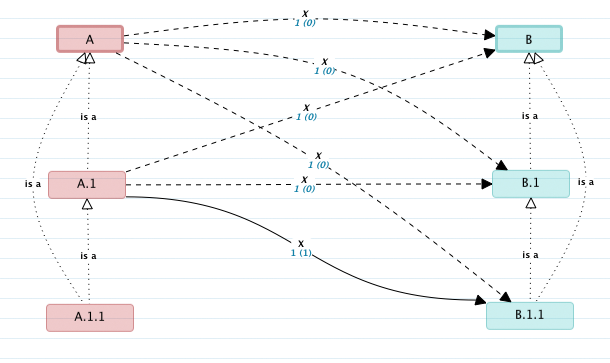
\includegraphics[width=1.0\linewidth]{Figures/proposed_relations1.png}
  \caption[APIUA: Modellierung --- Hypothetische Relationen I]{Die Relation \rel[x]{\code{apiua://code/-9223372036854774934}}{\code{apiua://code/-9223372036854774931}} ist in diesem ACM die einzige explizite Relation. Die übrigen mit gestrichelten Kanten dargestellten Relationen sind Vorschläge, die sich aus \rel[x]{\code{apiua://code/-9223372036854774934}}{\code{apiua://code/-9223372036854774931}} ergeben.}
  \label{fig:ProposedRelations1}
\end{figure}

\begin{figure}
  \centering
    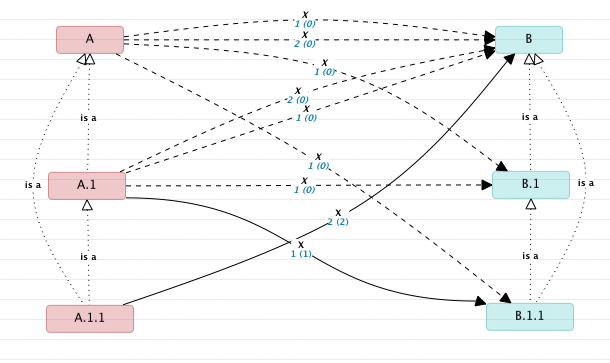
\includegraphics[width=1.0\linewidth]{Figures/proposed_relations2.png}
  \caption[APIUA: Modellierung --- Hypothetische Relationen II]{Dieses ACM unterscheidet sich von \ref{fig:ProposedRelations1} lediglich darin, dass es neben \rel[x]{\code{apiua://code/-9223372036854774934}}{\code{apiua://code/-9223372036854774931}} auch die Relation \rel[x]{\code{apiua://code/-9223372036854774932}}{\code{apiua://code/-9223372036854774935}} enthält. Daraus ergeben sich mehrere gleich lautende hypothetische Relationen zwischen denselben Konzepten (insb. zwischen \code{apiua://code/-9223372036854774936}~und~\code{apiua://code/-9223372036854774935}).}
  \label{fig:ProposedRelations2}
\end{figure}

\begin{figure}
  \centering
    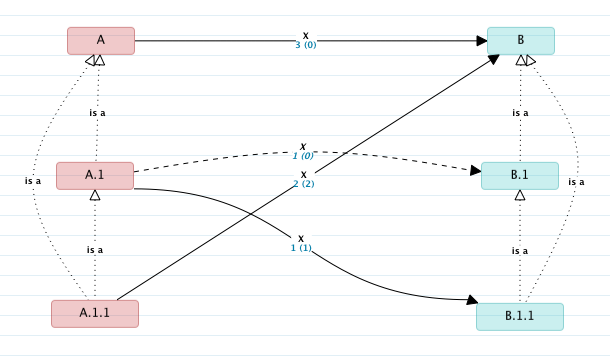
\includegraphics[width=1.0\linewidth]{Figures/proposed_relations3.png}
  \caption[APIUA: Modellierung --- Hypothetische Relationen III]{Im Gegensatz zu \ref{fig:ProposedRelations2} enthält dieses ACM zwischen \code{apiua://code/-9223372036854774936} und \code{apiua://code/-9223372036854774935} die explizite Relation \rel[x]{\code{apiua://code/-9223372036854774936}}{\code{apiua://code/-9223372036854774935}}. Dadurch entfallen alle hypothetischen Relationen, die in \code{apiua://code/-9223372036854774936} oder \code{apiua://code/-9223372036854774935} anfangen oder enden. Die einzig erhalten gebliebene hypothetische Relation ergibt sich aus \rel[x]{\code{apiua://code/-9223372036854774934}}{\code{apiua://code/-9223372036854774931}}.}
  \label{fig:ProposedRelations3}
\end{figure}

Informatisch gesehen ist das Produkt der Analyse, das hauptsächlich in den Phasen des offenen und axialen Kodierens entsteht, eine Ontologie --- also eine ``explizite Spezifikation einer Konzeptualisierung'' \citep{Gruber:1993jz}. Denn: Bevor der Forscher seine \acrlong{gt} in Form einer so genannten \textit{Story} erzählt, liegen lediglich \glspl{acm} vor, die man durch eine Ontologie beschreiben kann. Man könnte also auch vereinfacht(!) sagen, dass eine \acrlong{gt} auf einer rückwärts mit Hilfe synthetischen Schließens entwickelten Ontologie basiert, die in den Daten verankert ist bzw. ein Model für die Daten darstellt. Meiner Meinung nach eignet sich diese Beobachtung dazu, bessere Datenanalysewerkzeuge zu entwickeln, als es sie heute gibt.

Wenn man einmal von den im \sref{sec:gtm} angesprochenen terminologischen Ungereimtheiten der \gls{gtm} absieht, gibt es einen abgegrenzten Baukasten von Elementen (Konzepte, Eigenschaften, Kategorien, Relationen, etc.), aus denen die Grundlage der \gls{gt} besteht. Diese mögliche Anordnung dieser Elemente könnte man in einer Meta-Ontologie beschreiben. Ein \gls{gtm} geeignetes Datenanalysewerkzeug müsste dann nur noch diese Meta-Ontologie unterstützen und dem Forscher zur Verfügung stellen. Schließlich würde jede Ontologie, die ein Forscher entwickelt, eine Instanz dieser Meta-Ontologie sein.

Trifft man die Annahme, dass jede Theorie gewissen Gesetzmäßigkeiten unterliegt (z.B. Vererbung wie oben beschrieben), könnte man diese Interferenz- und Integritätsregeln ebenfalls in der Meta-Ontologie beschreiben. Auf diese Weise könnte ein Datenanalysewerkzeug Verletzungen der Ontologie an der Meta-Ontologie diagnostizieren und implizites Wissen durch Anwendung der Interferenzregeln explizit machen.

In \gls{apiua} sind Interferenzregeln wie hypothetische Relationen aktuell fest kodiert. Ideal wäre es, wenn Interferenzregeln selbst vom Anwender definiert und bedarfsweise, beispielsweise während Erkenntnisperspektivwechseln, (de)aktiviert werden könnten. Auf diese Weise müssten keine Gesetzmäßigkeiten mehr postuliert werden, die für alle Theorien gelten. Stattdessen hätte der Forscher die Möglichkeit, für seine \gls{gt} individuelle Regeln zu formulieren.

Ein ganz konkreter Anwendungsfall für individuelle Interferenzregeln könnte wie folgt lauten: Für fünf von sechs Unterkodes von Kode \code{apiua://code/-9223372036854774936} gilt die Relation \rel{\code{A\textsubscript{x}}}{\code{apiua://code/-9223372036854774935}}. Das Werkzeug könnte nun dem Anwender vorschlagen, zu prüfen, ob diese Relation möglicherweise auch für den sechsten Untercode von \code{apiua://code/-9223372036854774936} zutrifft und damit auf \rel{\code{apiua://code/-9223372036854774936}}{\code{apiua://code/-9223372036854774935}} verallgemeinert werden kann. Das Werkzeug sollte sich darüber hinaus die Grundlage dieser Entscheidung merken. Sollte später ein siebter Unterkode zu \code{apiua://code/-9223372036854774936} hinzukommen, gäbe es zwei Möglichkeiten: (1) Der Forscher prüft selbstständig, ob \rel{\code{apiua://code/-9223372036854774936}}{\code{apiua://code/-9223372036854774935}} auch für \rel{\code{A\textsubscript{7}}}{\code{apiua://code/-9223372036854774935}} gilt. (2) Das Datenanalysewerkzeug erkennt die veränderte Datenlage und fragt den Anwender aktiv. Die zweite Möglichkeit würde eine Umstrukturierungsoperation im Sinne der in \tref{tab:APIUARequirements} aufgezählten Anforderungen darstellen.

Die Krux ist, dass der Forscher im Sinne des \textit{ständigen Vergleichens} und der Güte seiner Forschungsergebnisse  dazu verpflichtet ist, die im Beispiel skizzierten Überlegungen anzustellen. Ich halte es aber für unwahrscheinlich, dass der Forscher diesem Anspruch bei hinreichend komplexen Abhängigkeiten innerhalb seiner Theorie ohne Werkzeugunterstützung genügen kann.

Diese von mir vorgeschlagenen Verbesserungen sind allerdings mit Vorsicht zu genießen, denn sie sind nicht ausgiebig erprobt. Im Rahmen der in dieser Arbeit präsentierten Forschung haben die implementierten Funktionen (Vererbung von Verankerungen; hypothetische Relationen; siehe \sref{sec:Datenanalyse-STL-Inkonsistenzen-vereinfachen}) zwar das axiale Kodieren deutlich vereinfacht. Dennoch kann man zu bedenken geben, dass allein der von einem Werkzeug stammende Vorschlag zur Änderung des eigenen Theoriemodells den Anwender auf eine Weise beeinflusst, auf die er ohne diese Hilfestellung nicht beeinflusst worden wäre. Ich kann nicht ausschließen, dass der unreflektierte Umgang mit derartigen Funktionen zu einer gewissen Starrheit/Rigidität auf Seiten des Forschers führen kann.

Meine ontologische Auseinandersetzung mit der \gls{gtm} an dieser Stelle war vornehmlich technisch gemeint. Sie möchte zum einen die Möglichkeit geben --- insbesondere im Rahmen von Open Science  --- Forschungsergebnisse menschen- aber auch maschinenlesbar zur Verfügung zu stellen. Das Potential dieses Vorgehens stellt auch \cite{MuhlmeyerMentzel:2011vs} heraus. Zum anderen möchte sie als Vorschlag für den Bau einer besseren Datenanalysesoftware verstanden werden. Die Abschätzung der Konsequenzen für eine derart entwickelte \gls{gt} kann diese Arbeit nicht leisten. Allein das Feld der \acrlong{gtm} mit seinen verschiedenen Strömungen \citep{Breckenridge:2012tf}, wie der klassischen \gls{gtm} von \cite{glaser1978theoretical}, der von \cite{strauss1990basics} oder der konstruktivistischen \gls{gtm} von \cite{charmaz2006constructing} ist dafür zu breit.



\subsection{Zusammenfassung}

In diesem Unterkapitel habe ich das für meine Forschung entwickelte Datenanalysewerkzeugs \gls{apiua} vorgestellt.

Qualitative Datenanalysewerkzeuge müssen große Datenmengen, verschiedenste Datenformate und alle Phasen bzw. Praktiken der \gls{gtm} unterstützen, um eine \gls{gt} von hoher Qualität nicht zu gefährden. Um einen wirklichen Mehrwert zu erzielen, müssen ebenso Umstrukturierungsoperationen und Analysefunktionen angeboten werden. Die Interoperabilität der Forschungsergebnisse erlaubt die Weiterverarbeitung durch andere Akteure der Forschungsgemeinde. 

\gls{apiua} verwendet zur Erfüllung dieser Anforderungen eine komponentenbasierte Drei-Ebenen-Architektur. Komponenten werden durch den Einsatz der \gls{rcp}, welche wiederum auf \gls{osgi} basiert, unterstützt. Das Werkzeug ist allgemein, aber insbesondere mit Hinblick auf die Unterstützung weiterer Datenformate, außerordentlich erweiterbar. Die \gls{gtm}-Komponente arbeitet ausschließlich mit \glspl{uri}, durch die jeder Datenpunkt eindeutig identifiziert wird. Auf diese Weise werden Funktionen wie das Kodieren von Daten oder das Schreiben von Memos einheitlich implementiert. Außerdem ist so das Werkzeug bei der Erfüllung der Gütekriterien \textit{Argumentative Interpretationsabsicherung} und \textit{Nähe zum Gegenstand} behilflich. 

\gls{apiua} erlaubt die Arbeit mit hoch strukturierten Daten. Die Anwendung wurde mit dem Anspruch entwickelt, selbst benutzerfreundlich zu sein. Dazu gehört unter anderem eine frei konfigurierbare Benutzeroberfläche, die ihren Zustand detailliert über mehrere Forschungssitzungen speichert und nicht --- im Gegensatz zu anderen Werkzeugen --- immer wieder neu hergestellt werden muss.

Im Unterschied zu \textit{ATLAS.ti} können in \gls{apiua} Kodes einfach gefiltert, intuitiv farbkodiert, sortiert und hierarchisch angeordnet werden. Trotz der überschaubaren Funktionalität wird axiales Kodieren in \gls{apiua} in einem konkurrenzlosen Umfang unterstützt.

Das Werkzeug unterstützt fest implementierte Interferenzregeln, die besonders beim axialen Kodieren hilfreich sind und bei \textit{ATLAS.ti} in keiner Weise angeboten werden. Eine Möglichkeit, frei konfigurierbare Interferenzregeln zu erlauben, erachte ich für außerordentlich wünschenswert. Eine Möglichkeit, dies zu erlauben, besteht darin, mit einer Meta-Ontologie zu arbeiten. Ich biete die Grundlage, auf der die zukünftige Forschung meine Überlegungen untersuchen kann.

Abgesehen vom Umbenennen unterstützt \textit{ATLAS.ti} keinerlei Umstrukturierungsoperationen. In der aktuellen Version bietet \gls{apiua} jedoch einige Funktionen, wie Operationen am Kodebaum und die Verallgemeinerung bzw. Zusammenfassung von Relationen. Umstrukturierungsfunktionen wie das Zusammenfassen oder Auftrennen von Kodes fehlen beiden Werkzeugen.

Weitergehende Analysefunktionen fehlen beiden Anwendungen ebenfalls. Eine Funktion zum Anzeigen von Kodes, die nur in wenigen Datenquellen auftauchen, wäre außerordentlich spannend. Mit dieser Information könnte der Forscher beispielsweise \textit{theoretisches Sampling} besser betreiben --- also exakter auswählen ob und welche Daten er noch erheben möchte, was wiederum der Erfüllung des Gütekriteriums \textit{Triangulierung} zuträglich wäre.

%Im \hyperref[sec:ausblick]{Ausblick} greife ich noch einmal die wichtigsten Punkte auf.

\bigskip

Der nächste Abschnitt befasst sich mit der eigentlichen \gls{gtm}-Analyse unter Verwendung des eben beschriebenen qualitativen Datenanalysewerkzeugs \acrlong{apiua}.